\chapter{Fundamentos de qu\'{\i}mica org\'anica}
El estudio de esta unidad parte de una revisi\'on del concepto de niveles de energ\'{\i}a electr\'onica; de acuerdo a los principios de la
teor\'{\i}a, se contin\'ua con el desarrollo de la noci\'on de orbital at\'omico y con la determinaci\'on de las configuraciones electr\'onicas
de los primeros veinte elementos. Se revisan los s\'{\i}mbolos electr\'onicos de Lewis, se relaciona la electronegatividad con los tipos de enlace:
i\'onico, covalente y covalente polar\index{enlace!covalente}. Se introduce el concepto de enlace covalente coordinado.

\section{Conceptos fundamentales}
\subsection{Niveles de energ\'{\i}a electr\'onica.}
No todos los electrones de un \'atomo se ubican a la misma distancia del n\'ucleo. Como hicieron notar la teor\'{\i}a de Bohr y la mec\'anica cu\'antica, la pro\-babilidad de encontrar a los electrones es m\'axima a determinadas distancias del n\'ucleo, que se llaman niveles de energ\'{\i}a. A los niveles de energ\'{\i}a tambi\'en se les llama capas electr\'onicas y pueden contener s\'olo un cierto n\'umero de ellos. Los niveles de energ\'{\i}a principales (\textbf{\gloss[word]{niveles}}) est\'an numeradas, comenzando con \textbf{n} = 1, para el nivel m\'as cercano al n\'ucleo, y continuando hasta  \textbf{n} = 7 para los elementos conocidos  (te\'oricamente, el n\'umero de niveles es infinito). Cada nivel sucesivo de energ\'{\i}a est\'a ubicado m\'as lejos del n\'ucleo. Los electrones en los niveles de energ\'{\i}a a distancias mayores tienen mayores energ\'{\i}as. El orden de cantidad de energ\'{\i}a de los \textbf{n}  niveles principales es: 

Niveles principales de energ\'{\i}a: $1< 2 < 3 < 4 < 5 < 6< 7$

El n\'umero de electrones que puede existir en cada nivel de energ\'{\i}a es limitado. El n\'umero m\'aximo de electrones para un determinado nivel de energ\'{\i}a puede calcularse con la f\'ormula 2\textbf{n}$^2$, siendo \textbf{n} el n\'umero del nivel principal de  energ\'{\i}a.

\begin{table}[hbt]
\caption[Electrones en el nivel principal de energ\'{\i}a]{N\'umero m\'aximo de
electrones que pueden ocupar en cada nivel principal de energ\'{\i}a.}
\label{tab1.cap3}
\begin{minipage}{\linewidth}
\begin{center}
\begin{tabular}{ cc }\hline
\textbf{Nivel principal} &\textbf{N\'umero m\'aximo de electrones en cada}\\
\textbf{de energ\'{\i}a}& \textbf{nivel de energ\'{\i}a,}$2n^2$\\ \hline
$1$&$2\times 1^2 = 2$\\
$2$&$2\times 2^2 = 8$\\
$3$&$2\times 3^2 = 18$\\
$4$&$2\times 4^2 = 32$\\
$5$&$2\times 5^2 = 50$\footnote{El valor te\'orico de $50$ electrones en el
nivel $5$ de energ\'{\i}a nunca se  ha alcanzado en elemento alguno conocido hasta la
fecha.}\\ \hline 
\end{tabular}
\end{center}
\end{minipage}
\end{table}


\subsection{Orbitales at\'omicos}\index{orbitales!atomicos@at�micos}
Los principales niveles de energ\'{\i}a contienen subniveles identificados con
las letras \textit{s,p,d} y \textit{f}. Se muestra una representaci\'on de los orbitales \textit{s} y \textit{p} en la \textbf{Figura~\ref{fig3:1}}.Estos \gloss[word]{orbitales} 
\index{orbitales} son aquellos en los que se localizan los electrones. El subnivel
\gloss[word]{subnivels} consiste en un orbital; el subnivel
\gloss[word]{subnivelp}  consiste en tres orbitales; el subnivel
\gloss[word]{subniveld} consta de cinco orbitales y el subnivel
\gloss[word]{subnivelf} consta de siete orbitales. Un electr\'on gira sobre su propio eje, lo que tambi\'en se le conoce como spin,  en uno de dos sentidos: en el sentido del reloj, y en el sentido contrario al del reloj. Cuando un or\-bital contiene dos electrones, se dice que los electrones est\'an en par o apareados. Como no pueden existir m\'as de dos electrones en un orbital, el n\'umero m\'aximo de electrones que puede existir en los subniveles son  2 en el orbital \textit{s}, 6 en los orbitales \textit{p}, 10 en los cinco orbitales \textit{d} y 14 en los siete orbitales \textit{f}.

\begin{table}[hbt]
\caption{Subniveles de energ\'{\i}a}
\label{tabla3.2}
\begin{center}
\begin{tabular}{ccc}\hline
\textbf{Tipo de} & \textbf{N\'umero posible}& \textbf{N\'umero posible}\\
\textbf{subnivel}& \textbf{de orbitales}  &\textbf{de electrones}\\\hline
\textit{s}&$1$&$2$\\
\textit{p}&$3$&$6$\\
\textit{d}&$5$&$10$\\
\textit{f}&$7$&$14$\\\hline
\end{tabular}
\end{center}
\end{table} 
El orden de de energ\'{\i}a dentro de un nivel principal es el si\-gui\-en\-te:  los electrones \textit{s} tienen menor energ\'{\i}a que los electrones \textit{p}
 y \'estos a su vez tiene menor energ\'{\i}a que los electrones \textit{d}, que son menos energ\'eticos que los electrones \textit{f}. Este orden se puede
expresar de la siguiente manera:
\begin{center}
Energ\'{\i}a del subnivel: \textit{s}$<$\textit{p}$<$\textit{d}$<$\textit{f}

\begin{figure}
\hspace{4cm}\resizebox{3cm}{3cm}{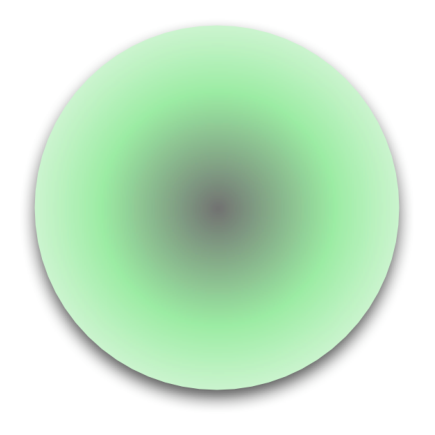
\includegraphics{orbitalS.eps}}
\vglue 0.2in
\hspace{1.5cm}\resizebox{9cm}{3cm}{ 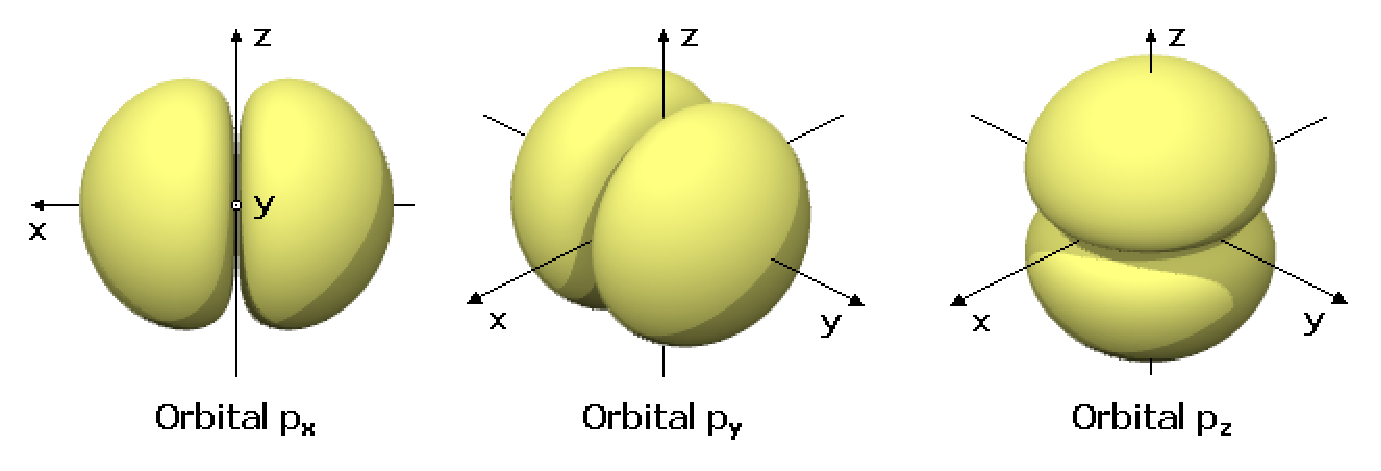
\includegraphics{orbitales_p.eps}}
%\vglue 0.05in
\caption[Orbitales $s$ y$p$]{Representaci\'on de un orbital tipo $s$ (parte superior)
y de un orbital $p$ (inferior)}
\label{fig3:1}
\end{figure}
\end{center}

\subsection{Configuraciones electr\'onicas}
Comenzando con el hidr\'ogeno y avanzando en el orden de n\'umero at\'o\-mi\-co
creciente, los \'atomos de helio, litio, berilio, etc., de cada uno de los elementos siguientes contiene un prot\'on y un electr\'on m\'as que los \'atomos
del elemento anterior.

Las estructuras electr\'onicas \index{estructuras@estructuras electr\'onicas} del  estado fundamental de los primeros 20 elementos quedan en un esquema regular. El
electr\'on \'unico del hidr\'ogeno est\'a en el primer nivel de energ\'{\i}a, como tambi\'en los dos electrones del helio. Las estructuras electr\'onicas para el
hidr\'ogeno y el helio son $1s^1$ y $1s^2$. El n\'umero m\'aximo de electrones en el primer de energ\'{\i}a es dos $(2n^2 = 2 \times 1^2 = 2)$. Por lo tanto, los dos
electrones llenan el primer nivel de energ\'{\i}a del helio.

Un \'atomo con tres electrones tendr\'a su tercer electr\'on en el segundo nivel de energ\'{\i}a, pues el primero s\'olo puede contener dos electrones. Por lo
anterior, el tercer electr\'on en el litio (n\'umero at\'omico 3) est\'a en el subnivel $2s$ del segundo nivel de energ\'{\i}a. El litio tiene la estructura
electr\'onica $1s^22s^1$. El \textbf{Cuadro~\ref{tabla3.3}} muestra la estructura electr\'onica de los primeros veinte elementos.

\begin{table}[ht]
\caption[Estructuras electr\'onicas]{Estructura electr\'onica de los primeros veinte
elementos}
\label{tabla3.3}
\begin{center}
{\small
 \begin{tabular}{lcl}\hline
\textbf{Elemento} & \textbf{N\'umero de} &\textbf{ Estructura} \\
    &       \textbf{electrones}& \textbf{electr\'onica}\\ \hline
H   &  1 & $1s^1$\\
He  &  2 & $1s^2$\\
Li  &  3 & $1s^22s^1$\\
Be  &  4 & $1s^22s^2$\\
B   &  5 & $1s^22s^22p^1$\\
C   &  6 & $1s^22s^22p^2$\\
N   &  7 & $1s^22s^22p^3$\\
O   &  8 & $1s^22s^22p^4$\\
F   &  9 & $1s^22s^22p^5$\\
Ne  & 10 & $1s^22s^22p^6$\\
Na  & 11 & $1s^22s^22p^63s^1$\\
Mg  & 12 & $1s^22s^22p^63s^2$\\
Al  & 13 & $1s^22s^22p^63s^23p^1$\\
Si  & 14 & $1s^22s^22p^63s^23p^2$\\
P   & 15 & $1s^22s^22p^63s^23p^3$\\
S   & 16 & $1s^22s^22p^63s^23p^4$\\
Cl  & 17 & $1s^22s^22p^63s^23p^5$\\
Ar  & 18 & $1s^22s^22p^63s^23p^6$\\
K   & 19 & $1s^22s^22p^63s^23p^64s^1$\\
Ca  & 20 & $1s^22s^22p^63s^23p^64s^2$\\ \hline 
\end{tabular}
}
\end{center}
\end{table}\index{estructuras@estructuras electr\'onicas!primeros veinte elementos} 

\subsection{S\'{\i}mbolos de Lewis}
El m\'etodo de puntos de Lewis para representar \'atomos propuesto por el qu\'{\i}\-mi\-co estadounidense G. N. Lewis \index{Lewis@\textbf{Lewis}!s\'{\i}mbolo}emplea el  s\'{\i}mbolo del elemento, y puntos gr\'a\-fi\-cos para representar electrones. El n\'umero de puntos que se colocan alrededor del s\'{\i}mbolo es igual al n\'umero de
electrones $s$ y $p$ del nivel externo de energ\'{\i}a del \'atomo. Los puntos pares representan electrones apareados, y viceversa, los puntos no en pares, electrones no apareados.
\newpage
\begin{example}
H$\cdot$ es el s\'{\i}mbolo de Lewis para un \'atomo de hidr\'ogeno, $1s^1$

 :\.B es el s\'{\i}mbolo de Lewis para un \'atomo de boro,
$1s^22s^22p^1$. En este caso el Boro  :\.B representa al n\'ucleo del
boro y a los electrones $1s^2$; los puntos representan s\'olo  a los
electrones $2s^22p^1$.
\end{example}

Cuando se tiene completa la capa de valencia con  ocho electrones se tiene un gas  \gloss[word]{gasesnobles}\index{gas!noble} que son un grupo de elementos qu\'{\i}micos con propiedades  similares. En condiciones normales de presi\'on y temperatura, son gases monoat\'omicos inodoros, incoloros y presentan muy poca reactividad qu\'{\i}mica.

\subsection{Energ\'{\i}a de ionizaci\'on y afinidad electr\'onica}

De acuerdo con el concepto de Bohr, existen electrones a varios niveles discretos de
energ\'{\i}a que dependen de la cantidad de energ\'{\i}a que ha absorbido el
\'atomo. Si se aplica suficiente energ\'{\i}a al \'atomo, es posible sacar
completamente (o expulsar) uno o m\'as electrones de su estructura, formando
as\'{\i} un ion positivo:
\begin{center}
\'atomo + energ\'{\i}a $\longrightarrow$ ion positivo + electr\'on (e$^-$)
\end{center}
La cantidad de energ\'{\i}a necesaria para quitar un electr\'on (e$^-$) a un \'atomo  a un ion se llama \textbf{energ\'{\i}a de \gloss[word]{ionizacion}}\index{energ\'{\i}a! de ionizaci\'on}. La energ\'{\i}a de \textit{primera} ionizaci\'on es la cantidad de energ\'{\i}a necesaria para sacar al primer electr\'on de un \'atomo; la energ\'{\i}a de \textit{segunda} ionizaci\'on es la necesaria para sacar al segundo electr\'on, y as\'{\i} sucesivamente.
\begin{table}
\caption[Energ\'{\i}as de ionizaci\'on]{Energ\'{\i}as de ionizaci\'on de algunos elementos}
\label{ionizacion}
\begin{center}
\begin{tabular}{l r r r r r}\hline
&\multicolumn{5}{c}{\textbf{Cantidades necesarias de energ\'{\i}a(kJ/mol)}}\\
\cline{2-6}
  Elemento &1o. e$^-$&2o. e$^-$&3o. e$^-$&4o.e$^-$&5o. e$^-$\\ \hline
H  &$1,314 $\\
He &$2,372 $& $5,247$\\
Li &$520   $& $7,297$ & $11,810$ \\
Be &$900   $& $1,757$ & $\mathbf{14,845}$ &$ 21,000$\\
B  &$800   $& $2,437$ & $ 3,657$ & $\mathbf{25,020}$&$ 32,810$\\
C  &$1,088$ & $2,352$ & $ 4,619$ &$  6,222$&  $\mathbf{37,800}$\\
Ne &$\mathbf{2,080}$ & $3,962 $& $ 6,376$ &  $9,376$& $ 12,190$\\
Na &$ 496$ & $\mathbf{4,565}$ & $ 6,912$ &  $9,540$&  $13,355$\\\hline
\multicolumn{6}{l}{\tiny Los valores se muestran en kilojoules por mol,
mostrando las energ\'{\i}as necesarias para sacar de}\\[-.1in]
\multicolumn{6}{l}{\tiny 1 a 5 electrones por \'atomo. 
Las negritas indica la energ\'{\i}a necesaria para sacar un electr\'on de
una}\\[-.1in]
\multicolumn{6}{l}{\tiny   estructura
electr\'onica de gas noble.}\\
\end{tabular}
\end{center}
\end{table}

Las energ\'{\i}a de ionizaci\'on se pueden expresar en t\'erminos de varias unidades de energ\'{\i}a, como electronvolts, kilojoules o kilocalor\'{\i}as por mol. En el siguiente ejemplo se expresa la energ\'{\i}a en kilojoule por mol (\kilo\joule/\mole), que indica el n\'umero de kilojoule necesarios para expulsar un electr\'on (e$^-$) de todos los \'atomos en un mol de \'atomos.
\begin{center}
\begin{tabular}{ccccccc}
Na &+& 494 \kilo\joule & $\longrightarrow$ &Na$^+$ &$+$ &e$^-$\\
{\scriptsize 1 mol de}&&&&{\scriptsize  1 mol de}&&{\scriptsize 1 mol de}\\[-.1in]
{\scriptsize \'atomos de sodio} &&&&{\scriptsize iones de sodio} & &{\scriptsize 
electrones}\\ 
\end{tabular}
\end{center}

El \textbf{Cuadro~\ref{ionizacion}} da las energ\'{\i}as de ionizaci\'on para la eliminaci\'on de uno a cinco electrones de varios elementos. As\'{\i} se necesitan 1314{\kilo\joule} para sacar un electr\'on de una mol de hidr\'ogeno, pero s\'olo se necesitan 494{\kilo\joule} para sacar el primer electr\'on de un mol de \'atomos de sodio. El \textbf{Cuadro~\ref{ionizacion}} muestra cantidades progresivamente mayores de energ\'{\i}a para expulsar al segundo, tercero, cuarto y quinto electrones. Esta secuencia es l\'ogica, por que la remoci\'on de electrones no disminuye al n\'umero de protones, o cantidad de carga, del n\'ucleo. Por lo tanto, los electrones restantes quedan sujetos m\'as fuertemente. El \textbf{Cuadro~\ref{ionizacion}} tambi\'en muestra que se necesita una energ\'{\i}a de ionizaci\'on extremadamente grande cuando se retira un electr\'on de una estructura de gas noble, lo cual demuestra la gran estabilidad de esa estructura.

En la tabla peri\'odica la energ\'{\i}a de primera ionizaci\'on disminuye generalmente con la colocaci\'on de arriba abajo, en cada una de las columnas conocidas como grupos  o familias.

De izquierda a derecha dentro de un per\'{\i}odo (o rengl\'on) de la tabla peri\'odica, la energ\'{\i}a de ionizaci\'on aumenta gradualmente, a pesar de algunas
irregularidades. Los gases nobles tienen valores relativamente altos, lo que confirma la no reactividad qui\'{\i}mica de esta familia y la estabilidad de una estructura de ocho electrones en el nivel externo de energ\'{\i}a.

Los \'atomos tienen \textbf{\gloss[word]{afinidadelectronica}}\index{afinidad!electronica@electr\'onica} -- esto es, capacidad para atraer electrones y formar iones negativos. \'Esta se puede definir como la cantidad de energ\'{\i}a absorbida o liberada cuando se agrega un electr\'on a un \'atomo para formar un ion negativo. Para la mayor parte de los elementos, se desprende calor cuando se agrega un electr\'on a un \'atomo.
\begin{center}
\'atomo + electr\'on $\longrightarrow$ ion negativo + energ\'{\i}a
\end{center}

La afinidad electr\'onica es una medida de la atracci\'on que ejerce un \'atomo  hacia un electr\'on -- en otras palabras, de la tendencia a formar un ion
negativo. El cloro, por ejemplo, es un elemento no met\'alico y tiene una fuerte tendencia a formar iones negativos. En consecuencia, la afinidad del cloro es alta.

\begin{tabular}{ccccccc}
Cl &+& e$^-$ & $\longrightarrow$& Cl$^-$ & + &384 {\kilo\joule}  (83 kcal)\\
{\scriptsize 1 mol de}&&{\scriptsize 1 mol de}&&{\scriptsize 1 mol de}\\[-.1in]
{\scriptsize \'atomos de cloro}&&{\scriptsize electrones}&&{\scriptsize iones
cloruro}\\
\end{tabular}

La afinidad electr\'onica tiende a ser alta en los no metales (en especial para los hal\'ogenos, ox\'{\i}geno y azufre) y baja en los metales. La tendencia general de la afinidad electr\'onica es aumentar de izquierda a derecha en cualquier periodo, y disminuir de arriba abajo en una familia de elementos.

\subsection[Electrones de valencia]{Electrones en la capa externa: electrones de
valencia}

Una propiedad importante de los elementos es su tendencia a formar una estructura con capa externa estable. Para muchos elementos, esta capa externa estable contiene ocho electrones (dos $s$ y seis $p$) que es id\'entica a la estructura electr\'onica externa de los gases nobles. Los \'atomos rearreglan su estructura electr\'onica para llegar a un estado de mayor estabilidad. Estos rearreglos se logran perdiendo, ganando o compartiendo electrones de otros \'atomos. Por ejemplo un \'atomo de hidr\'ogeno tiene la tendencia a aceptar otro electr\'on y as\'{\i} llegar a la estructura electr\'onica como la del gas noble helio; un \'atomo de fl\'uor puede adquirir un electr\'on m\'as para llegar a una estructura electr\'onica estable como la del ne\'on.

Los electrones en la capa externa de un \'atomo son responsables de la mayor parte de esta actividad electr\'onica, y se les llama \textbf{electrones de \gloss[word]{valencia}}\index{electrones de valencia}. En los s\'{\i}mbolos de Lewis con puntos, esos puntos representan los electrones de la capa externa, y por lo tanto tambi\'en representa a los electrones de valencia.

La regla del octeto\index{octeto!regla} es una regla pr\'actica que explica la formaci\'on del enlace qu\'{\i}mico de los elementos representativos en funci\'on de la configuraci\'on electr\'onica de su capa de valencia. Esta regla indica que, los \'atomos se combinan entre s\'{\i} de tal manera que cada \'atomo est\'e rodeado de ocho electrones en su capa de valencia (de all\'{\i} la denominaci\'on de ``octeto'').

\subsection[Electronegatividad y tipos de enlace]{Relaci\'on entre electronegatividad y tipos de enlace}


Cuando dos tipos diferentes de \'atomos comparten un par de electrones, un  \'atomo asume una carga parcial positiva y el otro una carga parcial negativa
entre s\'{\i}. Esta diferencia de cargas se representa porque los dos \'atomos  ejercen atracci\'on desigual hacia el par de electrones compartidos. La fuerza
de atracci\'on que un \'atomo de un elemento presenta hacia los electrones en  una mol\'ecula se llama \textbf{\gloss[word]{electronegatividad}}.
\index{electronegatividad} Los elementos difieren en sus electronegatividades. Por ejemplo, tanto el hidr\'ogeno como el cloro necesitan un electr\'on para formar
configuraciones electr\'onicas estables. Comparten un par de electrones en el cloruro de hidr\'ogeno. Como consecuencia, el par de electrones se desplaza hacia el
\'atomo de cloro, d\'andole una carga negativa parcial y dejando al \'atomo de hidr\'ogeno con una carga parcial positiva.

\subsubsection{Polaridad de enlace}
\'Atomos id\'enticos tienen electronegatividades id\'enticas. En la mol\'ecula
de hidr\'ogeno H$_2$  $$H:H$$ los \'atomos de hidr\'ogeno atraen por igual al par
electr\'onico. La distribuci\'on de carga electr\'onica es sim\'etrica con respecto
a los dos n\'ucleos; es decir, no est\'a m\'as cerca de un n\'ucleo que al otro. 
Como un enlace es e\-lec\-trost\'aticamente igual al otro, se dice que el enlace no
es \textit{polar}. \index{enlace!covalente!no polar} (Esto significa
exactamente que no tiene polos, o extremos diferentes). Por la misma raz\'on el
enlace  en la mol\'ecula del fl\'uor F:F es tambi\'en no polar. \textit{Los \'atomos
con electronegatividades id\'enticas forman enlaces covalentes no polares}.

Los \'atomos de diferentes elementos tienen diferentes electronegatividades. En la
mol\'ecula de fluoruro de hidr\'ogeno HF,  como el \'atomo de fl\'uor \textbf{F} tiene una
electronegatividad mayor que le del hidr\'ogeno \textbf{H}, el par electr\'onico est\'a
compartido desigualmente. La carga electr\'onica del par compartido est\'a m\'as
cerca del \'atomo de fl\'uor (el electr\'on se encuentra m\'as tiempo cercano al F que
al H). El enlace resultante tiene carga negativa acumulada en un extremo, y deja carga
positiva en el otro. (El n\'ucleo del hidr\'ogeno est\'a en el otro extremo y queda
en alguna forma expuesto por la p\'erdida de electrones). Un enlace covalente en el
cual el par electr\'onico es compartido desigualmente se dice que es un
\textit{enlace covalente polar} \index{enlace!covalente!polar}.

La \gloss[word]{polaridad} de un enlace, es decir, el grado al cual un par electr\'onico es desigualmente compartido, depende de la diferencia entre las
electrone\-gatividades de los dos \'atomos enlazados. Cuando la diferencia de las elec\-tro\-ne\-gatividades es grande, mayor es la polaridad en el enlace.

\subsubsection{Car\'acter i\'onico parcial}

 Cuando se enlazan dos \'atomos de gran diferencia de electronegatividad, el resultado se clasifica mejor como un enlace i\'onico. El enlace i\'onico puede considerarse como un enlace polar extremo, en el cual no se comparten esencialmente los electrones.\index{enlace!ionico@i\'onico}

En el \textbf{Cuadro~\ref{enlace}} se muestran las relaciones entre la diferencia de electronegatividad, el tipo de enlace, y grado de car\'acter i\'onico y covalente.
\index{enlace!covalente}
\begin{table}[thb]
\caption[Electronegatividades y enlaces]{Diferencia de electronegatividad, tipo y
car\'acter del enlace}
\label{enlace}
{\small \begin{tabular}{cccc}\hline
\textbf{Diferencia de}&&\textbf{Grado de car\'acter}&\textbf{Grado de car\'acter}\\
\textbf{electronegatividad}&\textbf{Tipo de enlace}&\textbf{Covalente}& 
\textbf{i\'onico}\\ \hline

Cero &Covalente no polar&$+$ & $-$ \\
   & $\downarrow$ &\\
 $\downarrow$ &Polar covalente&  $\downarrow$ & $\downarrow$ \\
  &  $\downarrow$ & \\
Grande & I\'onico & $-$ & $+$ \\ \hline
\end{tabular}}
\end{table}
\section {Alcanos, alquenos, alquinos y aro\-m\'a\-ti\-cos}

En esta secci\'on se estudian los principales grupos de hidrocarburos como son los 
alcanos, los alquenos, los alquinos y los aro\-m\'a\-ti\-cos. Se presenta el concepto de orbital
h\'{\i}brido co\-mo base para explicar la geometr\'{\i}a, la estructura y el
comportamiento qu\'{\i}mico de los compuestos de carbono. Se reconoce la estructura de
los alcanos, alquenos y alquinos con base en sus enlaces sencillos, dobles y triples, 
respectivamente. Se estudia con m\'as detenimiento la nomenclatura de los alcanos, ya
que \'esta sirve de base para los alquenos, alquinos y compuestos org\'anicos en
general.

Se muestrl fen\'omeno de isomer\'{\i}a que es caracter\'{\i}stico de los compuestos org\'anicos y se estudiar\'an las isomer\'{\i}as de cadena, de posici\'on y
geometr\'{\i}a (cis-trans).

La propiedades f\'{\i}sicas de alcanos, alquenos, alquinos y arom\'aticos se estudia en
forma global por tener propiedades semejantes.

\subsection{Hidrocarburos}
Los \textbf{\gloss[word]{hidrocarburos}} \index{hidrocarburos} son compuestos constituidos por \'atomos de carbono e hi\-dr\'o\-ge\-no unidos entre s\'{\i} mediante
enlaces covalentes. Se conocen varias clases de hidrocarburos. Esas clases son los alcanos, los alquenos, los al\-qui\-nos y los hidrocarburos arom\'aticos.

El benceno C$_6$H$_6$ es un hidrocarburo \textit{arom\'atico}.\index{benceno} Contiene
\'atomos de car\-bono en una estructura anular especial. Los compuestos que contienen el
 anillo del benceno se les conocen como\index{aromaticos@arom\'aticos}\textit{compuestos
arom\'aticos}. Se emplea el t\'ermino de \textit{\gloss[word]{alifatico}}\index{alif\'atico} para identificar compuestos con cadenas abiertas de \'atomos de
carbono. As\'{\i}, los alcanos, los alquenos y los alquinos de cadena abierta se les llama \textit{hidrocarburos alif\'aticos}. Los combustibles f\'osiles (gas natural,
petr\'oleo y carb\'on) son las principales fuentes de hidrocarburos. El gas natural es principalmente metano con pe\-que\-\~nas cantidades de etano, propano y butano. El petr\'oleo es una mezcla de hidrocarburos de la cual se separa la gasolina, el queroseno, el combust\'oleo, los aceites lubricantes, la parafina y el petrolato.

El alquitr\'an de hulla, que es un subproducto vol\'atil del proceso de fabricaci\'on de
coque a partir de carbones para la industria del acero, es fuente de muchas substancias
qu\'{\i}micas valiosas, incluyendo a compuestos arom\'aticos como el benceno, tolueno y
naftaleno.

\subsection{Hibridaci\'on del \'atomo de carbono}
\index{hibridacion@hibridaci\'on}
El carbono forma un sinn\'umero de compuestos en los que
sus \'atomos se enlazan covalentemente con otros cuatro \'atomos. el m\'as
simple de \'estos es el metano, CH$_4$. La configuraci\'on electr\'onica del
\'atomo de carbono en el estado fundamental es

\begin{center}
\begin{tabular}{rccccc}
C(Z=6):& $\underline{\uparrow \downarrow} $& $\underline{ \uparrow \downarrow}
$& $\underline{\uparrow \;} $ &$\underline{\uparrow \; }$
&$\underline{\quad}$\\[-.1in]
&&&\multicolumn{3}{c}{$\underbrace{\quad\quad\qquad\quad}$}\\
&$1s$&$2s$&\multicolumn{3}{c}{$2p$}\\
\end{tabular}
\end{center}
por esto el carbono aparece en capacidad de formar s\'olo dos enlaces covalentes
contribuyendo con cada uno de sus dos electrones no apareados para formar un par
compartido. Para la mol\'ecula de metileno (\ce{CH2}) de vida fugaz es mucho menos
estable que la de \ce{CH4}.

En la mol\'ecula de metano cada \'atomo de H est\'a localizado en la esquina de
un tetraedro regular. En el \ce{CH4} todas las longitudes de enlace son las mismas
y el \'angulo entre cada enlace \ce{C-H} y entre cada uno de los tres es el \textit{\'angulo
tetra\'edrico}, con un valor de $109.5^\circ$. 

El carbono evidentemente emplea todos sus cuatro electrones de valencia de modo
que puedan formarse cuatro enlaces C--H. No es demasiado dif\'{\i}cil ver c\'omo
el carb\'on forma cuatro enlaces. Suponga que uno de los dos electrones $2s$ es
promovido al orbital $2p$ vacante pero de mayor energ\'{\i}a.
\begin{center}
\begin{tabular}{rccccc}
C(Z=6):& $\underline{\uparrow \downarrow} $& $\underline{ \uparrow \;}
$& $\underline{\uparrow \;} $ &$\underline{\uparrow \; }$
&$\underline{\uparrow \;}$\\[-.1in]
&&&\multicolumn{3}{c}{$\underbrace{\quad\quad\qquad\quad}$}\\
&$1s$&$2s$&\multicolumn{3}{c}{$2p$}\\
\end{tabular}
\end{center}

Ahora el \'atomo de carbono est\'a en condiciones de formar cuatro enlaces $\sigma$ mediante la superposici\'on de sus orbitales $2s$ y $2p$ con los
orbitales $1s$ de los cuatro \'atomos de hidr\'ogeno. La dificultad aqu\'{\i} es que si el enlace ocurre de esa manera, la mol\'ecula de \ce{CH4} no ser\'{\i}a
tetra\'edrica. Si la estructura del metano determinada experimentalmente es tetra\'edrica ?`C\'omo podemos explicarla empleando los orbitales $s$ y $p$ del
carbono?. La respuesta es que el conjunto de orbitales $s$ y $p$ en el estado fundamental es reemplazado por un nuevo conjunto que es adecuado para formar
cuatro enlaces \textit{equivalentes}, cada uno en un \'angulo tetra\'edrico con respecto a los otros.

\gloss[nocite]{hibridacion}
Estos nuevos enlaces se les conoce como h\'{\i}bridos. Es la mezcla  o combinaci\'on de orbitales $s$ y $p$. El resultado es un orbital h\'{\i}brido, en el que la densidad de carga electr\'onica sufre un aumento. Este orbital h\'{\i}brido, llamado orbital\gloss[word]{orbitalsp}, es altamente direccional.

Podemos seguir la pista de la mezcla de los orbitales $2s$  y $2p$ en el carbono del siguiente modo:

\begin{tabbing}
\'Atomo en el estado fundamental \= $\qquad\underline{\uparrow \downarrow}\quad 
$\fbox{$\underline{\uparrow\downarrow}\quad
\underbrace{\underline{\uparrow\:\;}
\quad \underline{\uparrow\:\; }\quad \underline{\;\:\;}}$} \\
\>$\qquad 1s \quad\; 2s\quad \quad\quad 2p$\\
\>$\qquad \qquad \qquad \Downarrow$ {\footnotesize mezcla}\\
\'Atomo enlazado\>$\qquad\underline{\uparrow \downarrow}\quad 
$\fbox{$\underline{\uparrow \:\;}\quad
\underline{\uparrow \:\;}
\quad \underline{\uparrow\:\; }\quad \underline{\uparrow\:\;} $}\\
\>$\qquad 1s$  $\qquad \quad\quad 2sp^2$\\
\end{tabbing}
     
\subsection{Tipos de enlaces car\-bo\-no-car\-bono}\index{carbono!enlaces}
Con cuatro enlaces en la capa externa, el \'atomo de carbono siguiendo la regla del
octeto, forma cuatro enlaces sencillos covalentes compartiendo sus electrones con otros
\'atomos. Como ejemplo de \'esta tenemos las estruc\-turas del metano y del tetracloruro
de carbono un ejemplo de estos se muestra en la \textbf{Figura~\ref{fig3:2}}.

\begin{figure}[bht]
\hspace{1in} \resizebox{6cm}{6cm}{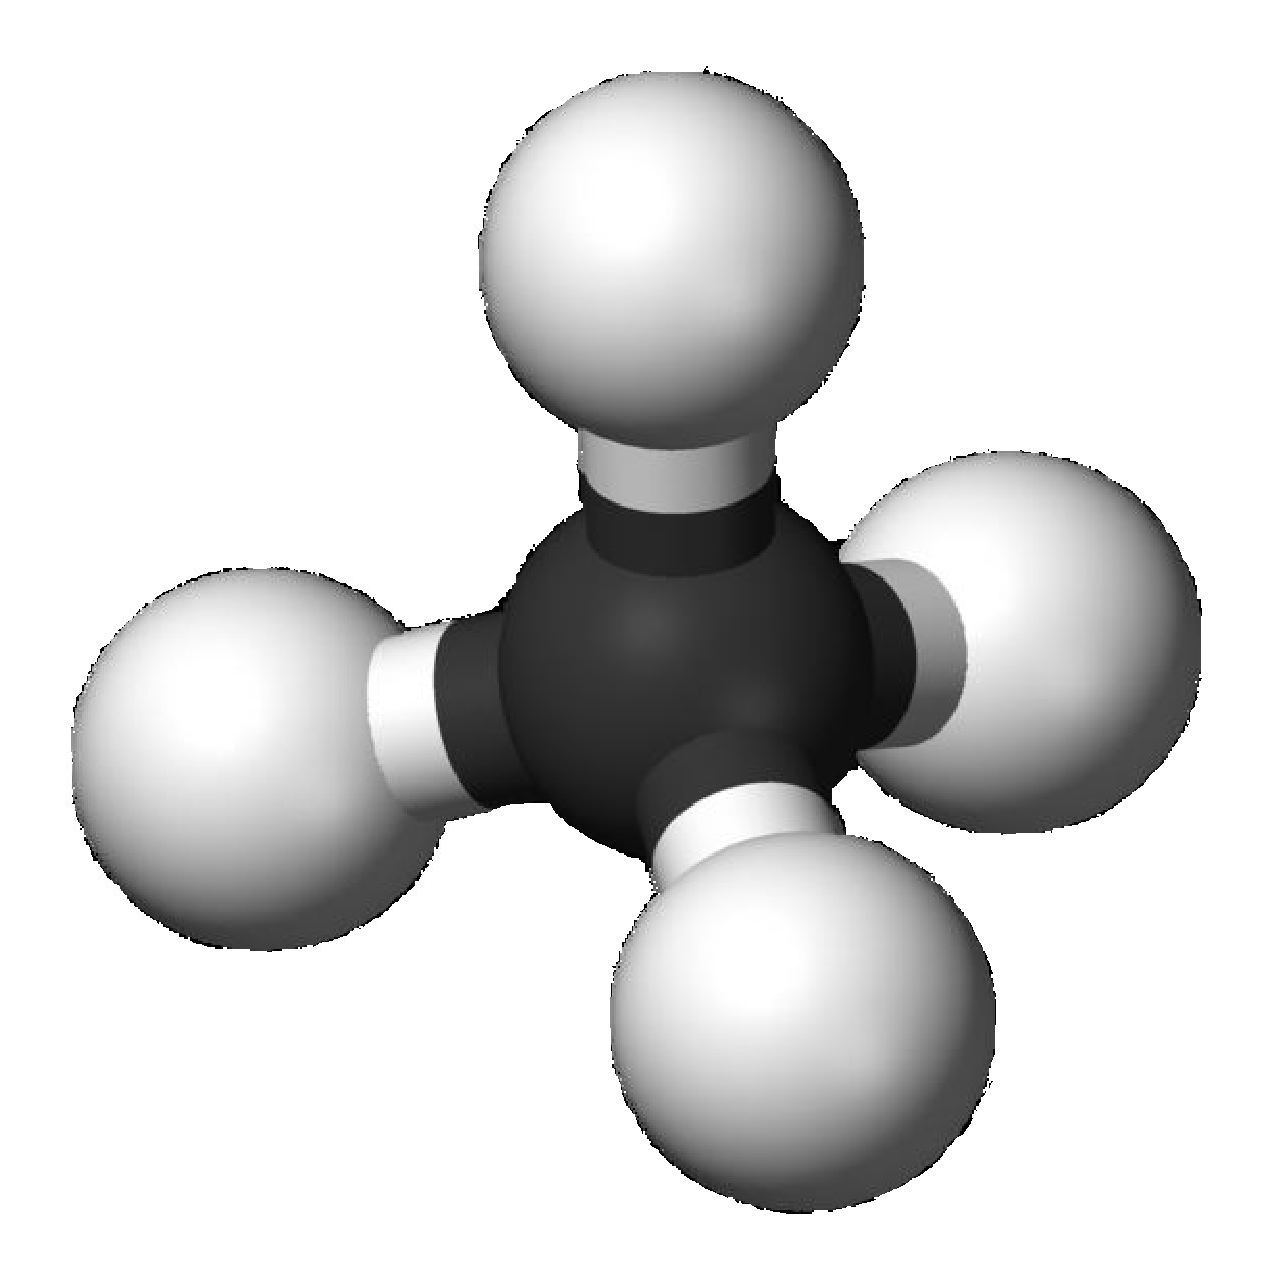
\includegraphics{metano3d.eps}}
\caption{Mol\'ecula de metano}
\label{fig3:2}
\end{figure}
En el metano, cada enlace se forma compartiendo electrones entre un \'atomo de carbono y un \'atomo de hidr\'ogeno.

La formaci\'on de los enlaces carbono-carbono se debe a la capacidad que tiene el \'atomo de carbono para compartir sus electrones con otros \'atomos iguales. Se pueden compartir uno, dos y tres pares de electrones entre dos \'atomos de carbono, formando respectivamente un enlace sencillo, un doble enlace y un triple enlace:
\begin{center}
\ce{C-C} \hskip .2in \ce{C\bond{2}C}  \hskip.2in  \ce{C\bond{3}C}  
\end{center}

Cada raya, en las f\'ormulas anteriores representa un enlace covalente. En el \textbf{Cuadro~\ref{enlaces}} se muestran algunos ejemplos de enlaces. El carbono, m\'as que ning\'un otro elemento, tiene la capacidad de formar cadenas de \'atomos enlazados covalentemente. Esta capacidad de enlazamiento es la principal raz\'on del gran n\'umero de compuestos org\'anicos.
\begin{center}
\begin{table}[htb]
\caption{Clases de compuestos org\'anicos}
\label{enlaces}
{\scriptsize \begin{tabular}{ l l l l l l }\hline
%\multicolumn{3}{l}{\textbf{clases de compuestos org\'anicos}}\\
& &Estructura& F\'ormulas &\multicolumn{2}{c}{\textbf{Nombre}}\\[-.01in]
 & F\'ormula &del grupo&estructurales\\[-.01in]
Clase   & general & funcional& de muestra& UIQPA$^a$ &Com\'un\\ \hline
Alcanos & RH &R$-$H & CH$_4$ &Metano & Metano\\
        &    &      & CH$_3$CH$_3$&Etano &Etano\\ \hline
Alquenos&R--CH$=$CH&$^\diagdown_\diagup $C$=$C$^\diagup_\diagdown$&CH$_2=$CH$_2$&
Etano & Etileno\\
       & &&CH$_3$CH$=$CH$_2$&Propeno&Propileno\\ \hline
Alquinos &R$-$\ce{CH\bond{3}C-H}& \ce{\bond{1}C\bond{3}C\bond{1}}&\ce{CH\bond{3}CH}&Etino &Acetileno\\
&&&CH$_3$C$\equiv$CH&Propino&Propileno\\
&&& &&Metilacetileno\\ \hline
Halogenuros&  &$-$X & CH$_3$Cl & Clorometano   &Cloruro de\\
de alquilo& &X$=$F,Cl, && &metilo\\
&&Br,I&CH$_3$CH$_2$Cl&Cloroetano &Cloruro de\\
&&&&& etilo\\[-.02in] \hline
\multicolumn{6}{l}{\scriptsize $^a$ IUPAC -- International Union of Pure and Applied Chemistry (Uni\'on Internacional de Qu\'{\i}mica Pura y Aplicada)}
\end{tabular}}
\end{table}
\end{center}

\subsection[Alcanos]{Hidrocarburos saturados: Alcanos}
Los \textbf{\gloss[word]{alcanos}}, \index{alcanos} son los hidrocarburos \textit{paraf\'{\i}nicos} o \textit{saturados}, estos compuestos tiene cadenas rectas o ramificadas de \'atomos de carbono, y entre dichos \'atomos s\'olo hay enlaces covalentes sencillos.
Estudiaremos con cierto detalle a los alcanos debido a que muchas otras clases de compuestos org\'a\-ni\-cos se les puede considerar como derivados de los alcanos. Por ejemplo, es necesario aprender los nombres de los primeros diez miembros de la serie de alcanos, por que tales denominaciones sirven de base para dar nombre a otras clases de compuestos.

\begin{table}[htd]
\caption[Alcanos caracter\'{\i}sticas]{Nombres, f\'ormulas y propiedades f\'{\i}sicas de los alcanos de cadena recta}
\label{alcanos}
\begin{center}
{\scriptsize \begin{tabular}{lllrr}\hline
 &\textbf{F\'ormula}& &\multicolumn{1}{c}{\textbf{Punto de}}
&\multicolumn{1}{c}{\textbf{Punto de}}\\
\textbf{Nombre} & \textbf{molecular} &&\multicolumn{1}{c}{\textbf{ebullici\'on}}&
\multicolumn{1}{c}{\textbf{fusi\'on}}\\ &
C$_n$H$_{2n+2}$&\multicolumn{1}{c}{\textbf{F\'ormula estructural condensada}}
&\multicolumn{1}{c}{($^\circ$C)}&\multicolumn{1}{c}{($^\circ$C)}\\
\hline
Metano &\ce{CH4}      & \ce{CH4}       &$-161$&$-183$\\
Etano  &\ce{C2H6}   &\ce{CH3CH3}&$-88$&$-172$\\
Propano&\ce{C3H8}  &\ce{CH3CH2CH3}&$-45$&$-187$\\
Butano &\ce{C4H10} &\ce{CH3CH2CH2CH3}&$-1$&$-138$\\
Pentano&\ce{C5H12} &\ce{CH3CH2CH2CH2CH3}&$36$&$-130$\\
Hexano &\ce{C6H14} &\ce{CH3CH2CH2CH2CH2CH3}&$69$&$-95$\\
Heptano&\ce{C7H16} &\ce{CH3CH2CH2CH2CH2CH2CH3}&$98$&$-90$\\
Octano &\ce{C8H18} &\ce{CH3CH2CH2CH2CH2CH2CH2CH3}&$125$&$-57$\\
Nonano &\ce{C9H20} &\ce{CH3CH2CH2CH2CH2CH2CH2CH2CH3}&$151$&$-54$\\
Decano &\ce{C10H22}&\ce{CH3CH2CH2CH2CH2CH2CH2CH2CH2CH3}&$174$&$-30$\\ \hline \hline
\end{tabular}}
\end{center}
\end{table}

El \textit{metano} (\ce{CH4})\index{metano} es el primer miembro de esta serie de alcanos.
Los miembros que tiene dos, tres y cuatro \'atomos son \textit{etano}, \textit{propano} y \textit{butano}, respectivamente. Los nombres de los primeros cuatro alcanos son de origen com\'un y se deben memorizar; pero los nombres de los dem\'as, comenzando con el del quinto miembro (\textit{pentano}), se derivan de nombres griegos para los n\'umeros y son relativamente f\'aciles de recordar. En el \textbf{Cuadro~\ref{alcanos}} se presentan los nombres, f\'ormulas y algunas propiedades de los primeros diez  miembros de la serie.

Los compuestos sucesivos en la serie de los alcanos difieren entre s\'{\i} en su composici\'on, por un \'atomo de carbono y dos de hidr\'ogeno. Cuando cada miembro de una serie difiere del siguiente por un grupo \ce{CH2}, a la serie se la llama \textbf{serie hom\'ologa} \index{serie hom\'ologa}. Los miembros de una serie hom\'ologa son semejantes en su estructura, pero tienen una diferencia regular en su f\'ormula. Para todos los alcanos de cadena abierta, la f\'ormula general es \ce{C_nH_{2n+2}}, siendo $n$ el n\'umero de \'atomos en la mol\'ecula.


\begin{example}

As\'{\i} para el pentano, $n=5$, y $2n+2=12$, de manera que la f\'ormula es \ce{C5H12} y para el hexadecano, que es un alcano con $16$ \'atomos de carbono, la f\'ormula es \ce{C16H34}.
\end{example}
\subsubsection{Estructuras e isomer\'{\i}a}

La estructura molecular determina algunas de las propiedades de una substancia qu\'{\i}mica. La estructura es el modo en el que los \'atomos se encuentran unidos
entre s\'{\i} en una mol\'ecula. La mayor parte de las mol\'eculas org\'anicas se forman con pocos elementos: carbono, hidr\'ogeno, ox\'{\i}geno, nitr\'ogeno y los
hal\'ogenos. En estos compuestos el carbono posee cuatro valencias (tetravalente), el hidr\'ogeno una  (monovalente), el ox\'{\i}geno dos (bivalente) y los ha\-l\'o\-ge\-nos son monovalentes. Una forma de representar los enlaces es mediante las ra\-yas o barras fijas a cada \'atomo:

\begin{center}
\begin{picture}(85,14)
%
\put(1,7.5){\line(1,0){3}}
\put(5,6){C}
\put(8.5,7.5){\line(1,0){3}}
\put(6.5,9.5){\line(0,1){2.5}}
\put(6.5,2.5){\line(0,1){2.5}}
%
\put(15,6){H}
\put(18,7.5){\line(1,0){3}}
%
\put(25,7.5){\line(1,0){3}}
\put(28,6){O}
\put(31.5,7.5){\line(1,0){3}}
%
\put(38,7.5){\line(1,0){3}}
\put(41,6){N}
\put(44.5,7.5){\line(1,0){3}}
%
\put(50,6){Cl}
\put(54,7.5){\line(1,0){3}}
%
\put(59,6){Br}
\put(63,7.5){\line(1,0){3}}
%
\put(69,6){I}
\put(70.5,7.5){\line(1,0){3}}
%
\put(76,6){F}
\put(78.5,7.5){\line(1,0){3}}
%
\end{picture}

\end{center}
As\'{\i}, el carbono tendr\'a cuatro enlaces para otros \'atomos; el nitr\'ogeno tres;  el ox\'{\i}geno dos; y los hal\'ogenos e hidr\'ogeno, uno.

En un alcano cada \'atomo de carbono est\'a unido a otros cuatro \'atomos mediante cuatro enlaces covalentes sencillos. Las mol\'eculas de alcano contiene s\'olo enlaces carbono-carbono y carbono-hidr\'ogeno, y son esencialmente no polares.

Debido a esta baja polaridad, las mol\'eculas de alcano tienen muy poca atracci\'on intermolecular, y por lo tanto sus puntos de ebullici\'on son relativamente bajos en
comparaci\'on con otros compuestos org\'anicos de masa molecular semejante.

Para expresar la f\'ormula estructural correcta para el propano (\ce{C3H8}) se debe  determinar c\'omo colocar cada \'atomo  en la mol\'ecula. Un alcano s\'olo contiene
enlaces sencillos, y el carbono es tetravalente. Por lo tanto, cada \'atomo de carbono debe estar enlazado a cuatro \'atomos m\'as mediante enlaces \ce{C-C} o \ce{C-H}. El hidr\'ogeno es univalente y por lo tanto se debe enlazar s\'olo a un \'atomo de carbono mediante un enlace \ce{C-H}, ya que no existen los enlaces \ce{C\bond{-}H-C}, y un enlace \ce{H-H} s\'olo representa una mol\'ecula de  hidr\'ogeno. Con esta informaci\'on se encuentra que la \'unica estructura posible para el propano es:
%
\begin{center}
\begin{picture}(40,20 )
%Hidrogenos de los extremos
\multiput(2, 8)(29,0){2}{H}
%Enlaces al centro
\multiput(6, 9.5)(7,0){4}{\line(1,0){3}}
% Carbonos al centro
\multiput(10, 8)(7,0){3}{C}
% Enlaces e Hidrogenos parte superior
\multiput(11.5,12)(7,0){3}{\line(0,1){2}}
\multiput(10,15)(7,0){3}{H}
% Enlaces e hidrogenos parte inferior
\multiput(11.5, 5)(7,0){3}{\line(0,1){2}}
\multiput(10, 1)(7,0){3}{H}
%
\end{picture}
\end{center}


Sin embargo, es posible trazar dos f\'ormulas estructurales que co\-rres\-ponden a la f\'ormula molecular \ce{C4H10}  (butano):
\begin{center}
\begin{picture}(92,40)
%  Cadena central
\multiput( 1,15)(36,0){2}{H}
\multiput( 5,16.5)( 7,0){5}{\line(1,0){3}}
\multiput( 9,15)( 7,0){4}{C}
%
%  Enlaces parte superior e Hidrogenos
%
\multiput(10.5,19)(7,0){4}{\line(0,1){2}}
\multiput( 9,22)(7,0){4}{H}
%
%  Enlaces parte inferior e Hidrogenos
%
\multiput(10.5,12)(7,0){4}{\line(0,1){2}}
\multiput( 9, 8)(7,0){4}{H}
%
\put(12,3){n-Butano}

%  Cadena central
\multiput(49,15)(29,0){2}{H}
\multiput(53,16.5)( 7,0){4}{\line(1,0){3}}
\multiput(57,15)( 7,0){3}{C}
%
%  Enlaces parte superior e Hidrogenos
%
\put(58.5,19){\line(0,1){2}}
\put(65.5,19){\line(0,1){5}}
\put(72.5,19){\line(0,1){2}}
%
\put(57,22){H}
\put(64,25){C}
\put(71,22){H}
%
%  Enlaces parte inferior e Hidrogenos
%
\multiput(58.5,12)(7,0){3}{\line(0,1){2}}
\multiput(57,8)(7,0){3}{H}

\put(65.5,29){\line(0,1){4}}
\put(64,34){H}
\put(63.5,27){\line(-4,5){3.3}}
\put(67.5,27){\line( 4,5){3.3}}
\put(58,32){H}
\put(70,32){H}
\put(56,3){iso-Butano}
\end{picture}
\end{center}

Se muestran los compuestos  C$_4$H$_{10}$ con las f\'ormulas estructurales que se
indican, y que en realidad existen. El butano con la cadena no ramificada de carbono se
llama
\textit{butano normal} (que se abrevia $n-$butano); hierve a 0.5 $^\circ$C y funde a
$-138^\circ$C. El  butano de cadena ramificada se lama \textit{isobutano}; hierve a$-
11.7^\circ$C, y funde a $-159.5^\circ$C. Estas diferencias hacen notar que aunque
tienen a misma f\'ormula molecular, son substancias distintas.

El fen\'omeno en el que dos o m\'as compuestos tiene la misma f\'ormula molecular, pero
diferente arreglo en los \'atomos, se llama \textbf{isomerismo}. A los diferentes
compuestos con la misma f\'ormula se les conoce como \textbf{\gloss[word]{isomeros}}. 
\index{is\'omeros} El isomerismo es com\'un en los compuestos org\'anicos y es uno de
los motivos del gran n\'umero de compuestos conocidos. Hay tres is\'omeros del pentano,
5 is\'omeros del hexano, 9 is\'omeros del heptano, 18 is\'omeros del octano, 35 del
nonano y 75 del decano.

Para ahorrar tiempo y espacio en la escritura, se emplean con frecuencia las f\'ormulas
\textit{condensadas}.  En las f\'ormulas estructurales condensadas, los
\'atomos y grupos que est\'an fijos a un \'atomo de carbono se escriben a la derecha de
ese \'atomo.

  Por ejemplo la f\'ormula condensada del pentano es:

CH$_3$CH$_2$CH$_2$CH$_2$CH$_2$CH$_3$, o tambi\'en CH$_3($CH$_2)_3$CH$_3$

\subsubsection{Nomenclatura}\index{Nomenclatura!alcanos}\index{alcanos!nomenclatura}

Para asignarle un nombre a un compuesto al principio lo hac\'{\i}a quien lo hab\'{\i}a
sintetizado. Estos nombres no segu\'{\i}an alguna secuencia o sistematizaci\'on. Por
ejemplo el metano, se forma durante la descomposici\'on de la materia org\'anica en las
marisma o pantanos, as\'{\i} se le llam\'o como el \textit{gas de los pantanos}. Debido
a esto, a un solo compuesto se le asignaban diferentes nombres. De esta forma tenemos al
alcohol de las bebidas que se le conoce como \textit{alcohol}, \textit{alcohol
et\'{\i}lico, metil-carbinol, alcohol de granos, esp\'{\i}ritu de vinos} y
\textit{etanol.}\index{etanol}\index{alcohol}

A partir de una convenci\'on en Ginebra, el a\~no de 1892, se desarroll\'o un sistema internacional de nomenclatura de compuestos.

\begin{table}[hbt]
\caption[Grupos alquilo]{Nombres y f\'ormulas de algunos grupos alquilo}
\label{a-nom}
\begin{center}
\begin{tabular}{ll l l}\hline
\multicolumn{1}{c}{\textbf{F\'ormula}}&\multicolumn{1}{c}{\textbf{Nombre}}&
 \multicolumn{1}{c}{\textbf{F\'ormula}}&\multicolumn{1}{c}{\textbf{Nombre}}\\ \hline
CH$_3-$                & Metilo  &CH$_3($CH$_2)_4$CH$_2-$ & Hexilo \\
CH$_3$CH$_2-$          & Etilo   &CH$_3($CH$_2)_5$CH$_2-$ & Heptilo \\
CH$_3$CH$_2$CH$_2-$    & Propilo &CH$_3($CH$_2)_6$CH$_2-$ & Octilo \\
CH$_3($CH$_2)_2$CH$_2-$& Butilo  &CH$_3($CH$_2)_7$CH$_2-$ & Nonilo \\
CH$_3($CH$_2)_3$CH$_2-$& Pentilo &CH$_3($CH$_2)_8$CH$_2-$ & Decilo \\\hline
\end{tabular}
\end{center}
\end{table}
Para asignar sistem\'aticamente los nombres a los compuestos org\'anicos, es necesario  reconocer ciertos grupos \gloss[word]{alquilo} comunes. Los \textbf{grupos alquilo} \index{grupo!alquilo} tienen la f\'ormula general C$_n$H$_{2n+1}$ (teniendo un \'atomo menos de hi\-dr\'o\-ge\-no que el alcano correspondiente). Para obtener el nombre del grupo que se forma se usa el nombre del alcano correspondiente, se elimina su
terminaci\'on \textit{ano} y se sustituye por la terminaci\'on \textit{ilo}. En el \textbf{Cuadro~\ref{a-nom}} se dan  los nombres y f\'ormulas de algunos grupos alquilo. Com\'unmente se emplea la letra ``\textbf{R}'' en las f\'ormulas para indicar a cualquiera de los grupos alquilo posibles.

\hskip1.5in R = \ce{C_nH_{2n+1}} \hspace{.2in} (grupo alquilo)

Las siguientes reglas\index{Nomenclatura!reglas UIQPA} son las que se necesitan para dar
nombre a una gran cantidad de alcanos de acuerdo a el sistema
\gloss[short]{UIQPA} \footnote{Uni\'on Internacional de Qu\'{\i}mica Pura y Aplicada}. Y
son como sigue:
\begin{enumerate}
\item Seleccionar la cadena continua m\'as larga de \'atomos de carbono como compuesto
padre, y considerar a los otros grupos alquilo fijos a ella como cadenas de
ramificaci\'on o sustituyentes que han reemplazado a \'atomos de hidr\'ogeno del
hidrocarburo progenitor. Si se encuentran dos cadenas de igual longitud, se emplea la
que tiene mayor n\'umero de sustituyentes fijos a ella. El nombre del alcano
corresponde del nombre del compuesto originalmente precedido por los nombres de los
grupos alquilo fijos a \'el.
\item Numerar los \'atomos de carbono de la cadena del compuesto padre, comenzando por el
extremo m\'as pr\'oximo al primer \'atomo de carbono que contenga fijos a \'el un grupo
alquilo u otro grupo funcional, sustituyendo a  un \'atomo de hidr\'ogeno. Si el primer
sustituyente a partir de cada extremo queda en el carbono con el mismo n\'umero, se
procede hacia el siguiente sustituyente para determinar qu\'e extremo de la cadena se
emplea para comenzar la numeraci\'on.
\item Se da el nombre a cada grupo alquilo y se especifica su posici\'on en la cadena
de carbonos del compuesto padre mediante un n\'umero (por ejemplo: 3-metil significa un
grupo metilo fijo al C n\'umero 3).
\item Cuando se presenta la cadena fija ramificada con el mismo grupo  alquilo m\'as de
una vez, se indica esa repetici\'on con un prefijo (\textit{di}, \textit{tri},
\textit{tetra}, y as\'{\i} sucesivamente) escrito frente  al nombre del grupo alquilo
(por ejemplo, dimetil indica que existen dos grupos metilo).  Los n\'umeros indican las
posiciones de esos grupos alquilo se separan por na coma y se siguen de un gui\'on,
anteponi\'endolos al nombre (p.e. 2,3-dimetil).
\item Cuando existen varios grupos alquilo diferentes fijos al compuesto progenitor, se
enuncian en orden alfab\'etico. Por ejemplo, el etil antes que el metil en el
3-etil-4-metiloctano. Los prefijos no se consideran en el ordenamiento alfab\'etico
(etil viene antes de dimetil).
\end{enumerate}

Al compuesto siguiente se le llama generalmente isopentano. Su denominaci\'on de
acuerdo con el sistema UIQPA ser\'a como sigue:

\begin{picture}(110,16)
\put( 1,9){CH$_3$}
\put( 9,10.5){\line(1,0){3}}
\put(13,9){CH$_2$}
\put(21,10.5){\line(1,0){3}}
\put(25,9){CH}
\put(32.5,10.5){\line(1,0){3}}
\put(37,9){CH$_3$}
\put(25,2){CH$_3$}
\put(26.5,6){\line(0,1){2}}

\put(50,9){o bien}
\put(45,2){\scriptsize 2-Metil butano}
\put(66,9){CH$_3$}
\put(74,10.5){\line(1,0){3}}
\put(78,9){CH}
\put(86,10.5){\line(1,0){3}}
\put(90,9){CH$_2$}
\put(98 ,10.5){\line(1,0){3}}
\put(102,9){CH$_3$}
\put(78,2){CH$_3$}
\put(79.5,6){\line(0,1){2}}

\setcounter{cm}{5}
\multiput( 2,13)(12,0){4}{\addtocounter{cm}{-1}
  \makebox(0,0)[b]{{\scriptsize \arabic{cm}}}}
\setcounter{cm}{0}
\multiput(67,13)(12,0){4}{\addtocounter{cm}{ 1}
  \makebox(0,0)[b]{{\scriptsize \arabic{cm}}}}
\end{picture}

La cadena continua m\'as larga contiene cuatro \'atomos de carbono. Por lo tanto, el compuesto padre es el butano y el compuesto se denomina como un derivado del butano. El grupo metilo (\ce{CH3}--)\index{metilo} fijo al carbono n\'umero 2 se usa como prefijo del butano, y el
``2'' indica el punto de fijaci\'on del grupo en la cadena but\'anica.

\subsection[Alquenos y Alquinos]{Hidrocarburos insaturados: Alquenos y alquinos}

Gran parte de los compuestos org\'anicos se sintetizan a partir de materiales
iniciales como: etileno, propileno, benceno, butileno, tolueno, xileno y metano. De esas
siete substancias mencionadas, todas, con excepci\'on del etano, son hidrocarburos no
saturados. tan s\'olo el etileno es la base de casi la mitad de los productos
petroqu\'{\i}micos.

Tanto los \textbf{\gloss[word]{alqueno}}\index{alquenos} y los
\textbf{\gloss[word]{alquino}} \index{alquinos} son hidrocarburos no saturados. Se
les dice no saturados, porque a diferencia de los alcanos, sus mol\'eculas no
contienen el n\'umero m\'aximo posible de \'atomos de hidr\'ogeno. Los alquenos tiene
dos \'atomos menos de hidr\'ogeno, y los alquinos tiene cuatro menos que los
correspondientes alcanos. Los alquenos (tambi\'en conocidos como hidrocarburos
\textit{olef\'{\i}nicos}) contiene al menos un doble enlace entre \'atomos de C
adyacentes. Los alquinos (\textit{acetil\'enicos}) contiene al menos un triple enlace
entre \'atomos adyacentes de carbono.

\subsubsection{Estructura}

El etileno (o eteno) es el alqueno m\'as simple, CH$_2=$CH$_2$, y el alquino m\'as
sencillo es el acetileno (o etino), \ce{CH\bond{3}CH}, (\textbf{F\/igura~\ref{fig3:3}}). El etileno y el
acetileno son los primeros miembros en las series hom\'ologas en las que las f\'ormulas
de los miembros sucesivos difieren por incrementos de CH$_2$. Por ejemplo,
\ce{CH2\bond{2}CH2}, \ce{CH3CH\bond{2}CH2} y \ce{CH3CH2CH\bond{2}CH2}.

\begin{figure}[htb]
\hspace{.5cm}\resizebox{6cm}{4cm}{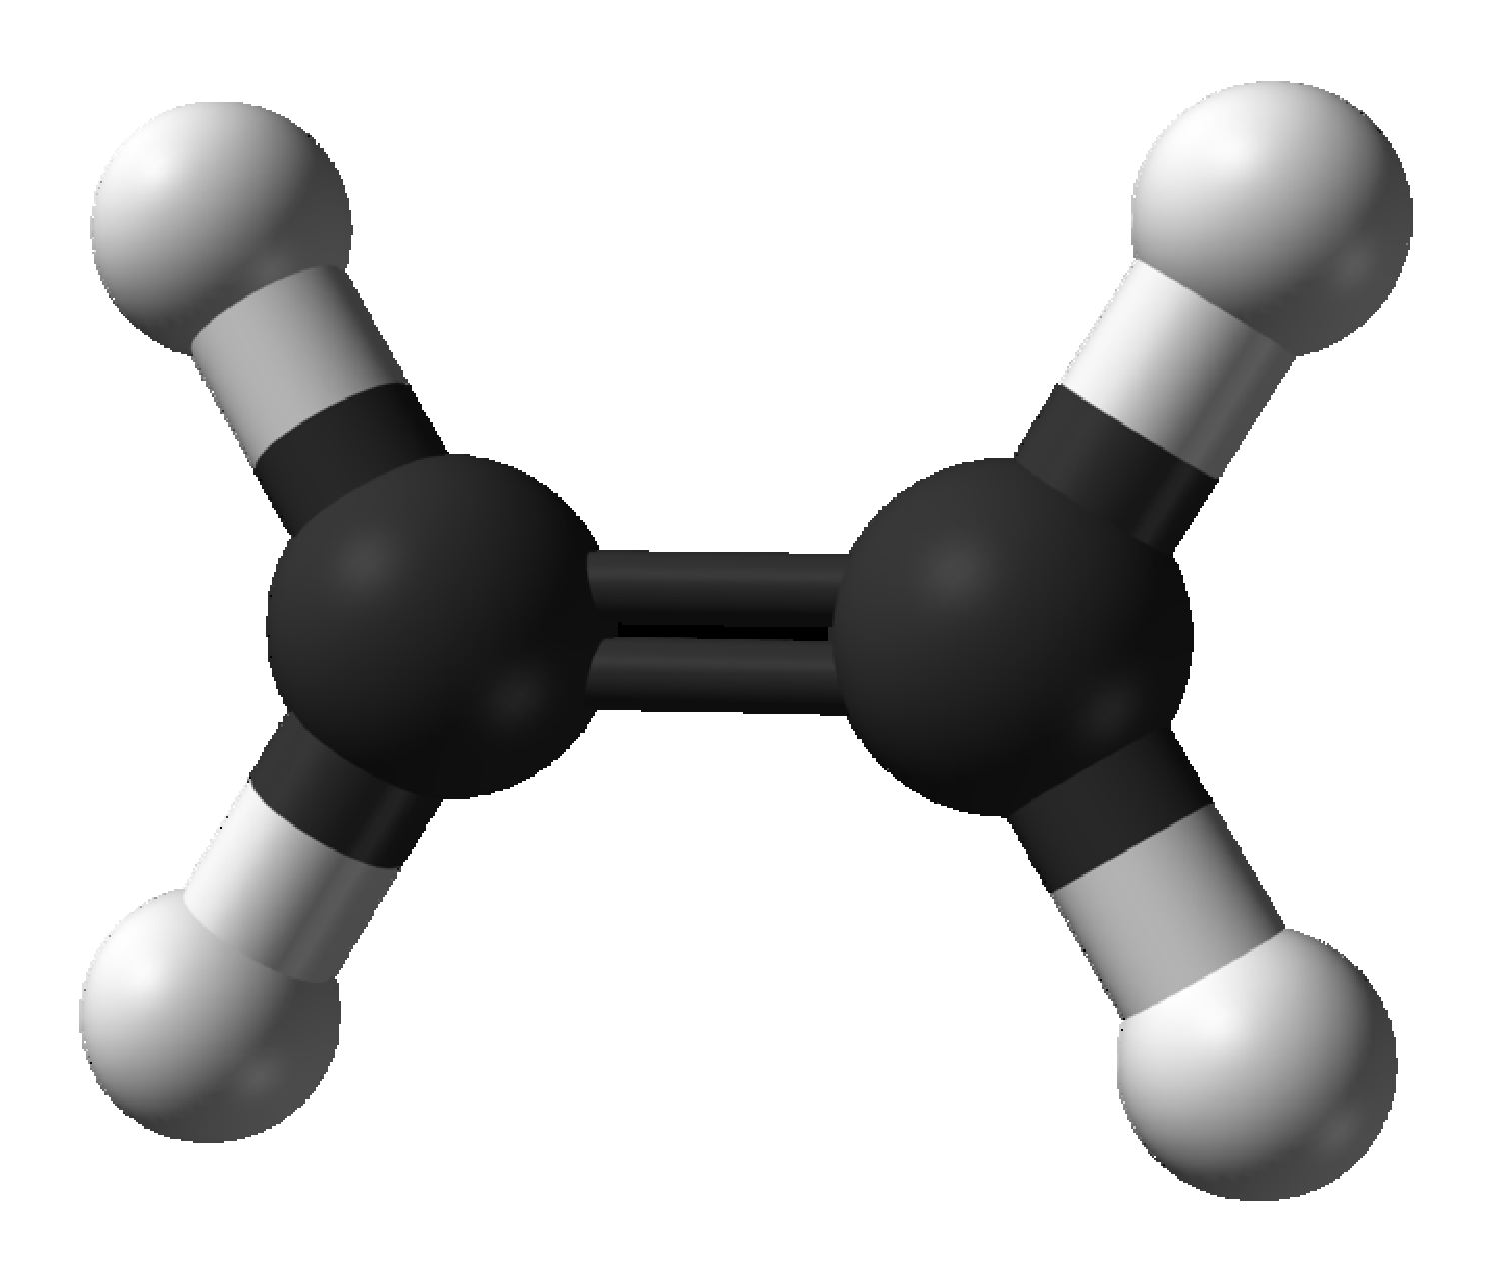
\includegraphics{etileno.eps}}
\resizebox{6cm}{2cm}{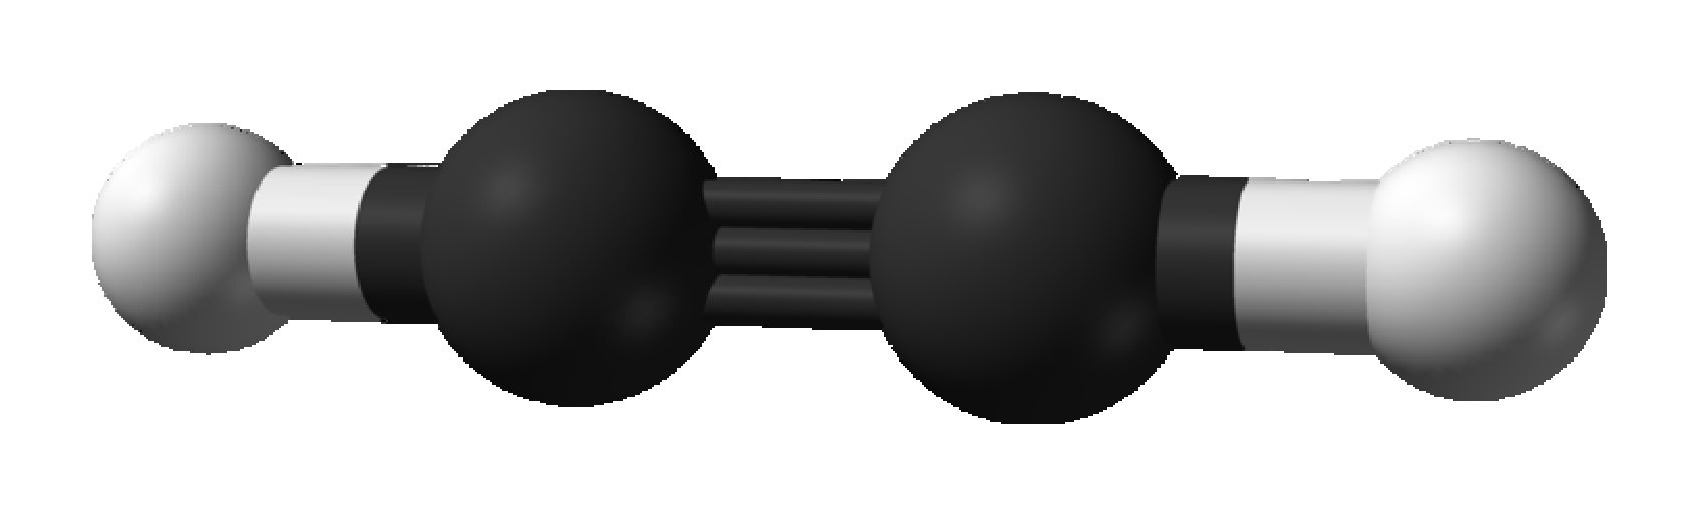
\includegraphics{acetileno.eps}}
\caption[Mol\'eculas de etileno y acetileno]{Mol\'eculas de etileno (izq.) y acetileno (der.)}
\label{fig3:3}
\end{figure}

\subsubsection{Propiedades f\'{\i}sicas}

Las mol\'eculas de los alquenos, como las de los alcanos, tienen muy poca polaridad. Por lo tanto, las propiedades f\'{\i}sicas de los alquenos son muy semejantes a las de los correspondientes hidrocarburos saturados. Los alquenos que contienen dos a cuatro \'atomos de carbono son gases; los que tiene 5 a 18 \'atomos de carbono son l\'{\i}quidos; y los que tiene m\'as de 18 carbonos son s\'olidos. Son relativamente poco solubles en agua, pero se disuelven en \'acido sulf\'urico concentrado. En el \textbf{Cuadro~\ref{prop:1}} se resumen algunas de la propiedades de los alquenos m\'as comunes.

\begin{table}[hbt]
\caption[Propiedades de Insaturados]{Propiedades f\'{\i}sicas de varios alquenos y alquinos}
\label{prop:1}
\begin{center}
{\small \begin{tabular}{lr r}\hline
&\multicolumn{1}{c}{\textbf{Punto de}}&
\multicolumn{1}{c}{\textbf{Punto de }}\\ 
&\multicolumn{1}{c}{\textbf{ fusi\'on}}&
\multicolumn{1}{c}{\textbf{ ebullici\'on}}\\
\multicolumn{1}{c}{\textbf{Compuesto}} &\multicolumn{1}{c}{$^\circ$\textbf{C}}&
\multicolumn{1}{c}{$^\circ$\textbf{C}}\\\hline
 Etileno &                  $-169$& $-104$\\
 Propileno&               $-185$& $-48$ \\
1-Buteno&                 $-185$& $-6$\\
2-Buteno (\textit{cis})&  $-139$& $+4$ \\
2-Buteno (\textit{trans})&$-106$& $+1$ \\
1-Penteno                &$-165$& $+30$ \\
1-Hexeno                & $-140$& $+64$\\
ciclo penteno           &$-135$& $+44$\\
 Acetileno                 &$  -82$& $-57$\\
 Propino                   &$-103$& $-23$\\
 1-Butino                  &$-126$& $+8$\\
2-Butino                 &$   -32$& $+27$\\ 
1-Pentino                &$-106$& $+40$\\
2-Pentino                &$-109$& $+56$\\
1-Hexino                 &$-132$& $+71$\\
2-Hexino                 &$  -90$& $+84$\\
\hline \hline
\end{tabular}}
\end{center}
\end{table}


\subsubsection{Nomenclatura}
\index{alquenos!nomenclatura}
\index{alquinos!nomenclatura}
\index{Nomenclatura!alquenos}
\index{Nomenclatura!alquinos}

Se fabrican grandes cantidades de alquenos por desintegraci\'on (o \gloss[word]{craqueo}) y \index{craqueo} deshidrogenaci\'on\index{deshidrogenacion@deshidrogenaci�n}  de alcanos en el procesamiento de petr\'oleos crudos. 

En el \textbf{Cuadro~\ref{insat:1}} da los nombres de las f\'ormulas para varios alquenos y alquinos comunes.
\begin{table}[htb]
\caption[Grupos Insaturados]{Nombres y f\'ormulas de varios alquenos y alquinos}
\label{insat:1}
\begin{center}
{\small \begin{tabular}{lll}\hline
\multicolumn{1}{c}{\textbf{F\'ormula}}&\multicolumn{1}{c}{\textbf{Nombre UIQPA}}&
\multicolumn{1}{c}{\textbf{Nombre com\'un}}\\ \hline
\ce{CH2\bond{=}CH2}                 & Eteno & Etileno\\
\ce{CH3-CH\bond{=}CH2}          &Propeno  & Propileno\\
\ce{CH3-CH2-CH\bond{=}CH2}   & 1-Buteno & Butileno\\
\ce{CH3-CH\bond{=}CH-CH3}     & 2-Buteno \\
\\
\ce{CH\bond{3}CH}                  & Etino & Acetileno \\
\ce{CH3-C\bond{3}CH}   & Propino  &  Metilacetileno\\
\ce{CH3-CH2-C\bond{3}CH} & 1-Butino & Etilacetileno\\
\ce{CH3-C\bond{3}C-CH3}& 2-Butino & Dimetilacetileno\\ \hline \hline

\end{tabular}}
\end{center}
\end{table}

Los nombres de los alquenos y alquinos se derivan de los nombres de los correspondientes alcanos. Para dar nombre a un alqueno (o alquino) de acuerdo con el sistema UIQPA:

\begin{enumerate}
\item Se selecciona la cadena carbono-carbono m\'as larga que contenga al doble o triple enlace.
\item Se nombra al compuesto padre obteniendo como si se tratara de un alcano, pero se cambia la terminaci\'on \textit{ano} por la terminaci\'on \textit{eno}, si se trata de un alqueno, o \textit{ino} para un alquino. Por ejemplo el propano cambia a propeno o a propino:

{\scriptsize \begin{tabular}{ccc}
\ce{CH3-CH2-CH3}& \ce{CH3-CH\bond{=}CH2}    &\ce{CH3-C\bond{3}CH}  \\
\textit{Propano} & \textit{Propeno} &\textit{Propino}\\
\end{tabular}}

\item Se numera la cadena de carbonos del compuesto progenitor comenzando con el extremo m\'as cercano al doble o triple enlace. Se usa el menor de los dos n\'umeros que se obtengan en los \'atomos con el doble o el triple enlace. Se coloca este n\'umero frente al nombre del alqueno o alquino; por ejemplo, 2-buteno que quiere decir que el doble enlace carbono-carbono se encuentra entre C-2 y C-3.

\item Las cadenas laterales y dem\'as grupos se tratan como cuando se dan nombres a los alcanos. Se nombra el grupo sustituyente, y se especifica su posici\'on en la cadena principal como n\'umero.

\end{enumerate}

\subsubsection{F\'ormulas generales} Para describir tanto los alquenos como los alquinos se pueden utilizar ecuaciones condensadas generales como las siguientes:

La f\'ormula general de alquenos es: \textbf{C}$_n$\textbf{H}$_{2n}$

La f\'ormula general de alquinos es:  \textbf{C}$_n$\textbf{H}$_{2n-2}$

\begin{exercises}
\exer  Nombra los siguientes compuestos:
\begin{figure}[ht]
\sidebyside{
\begin{picture}(50,16)
\put( 1,12){(a) CH$_3$CHCH}

\put(14,9){\line(0,1){2}}
\put(13.5,5){CH$_3$}

\put(24.5,12.5){\line(1,0){3}}
\put(24.5,13.5){\line(1,0){3}}
\put(29,12){CHCHCH$_3$}
\put(35,9){\line(0,1){2}}
\put(34.5,5){CH$_2$CH$_3$}
\put(12,0){{\scriptsize Resp:  (a) 2,5-dimetil-3-hepteno }}
\end{picture}
}
{
\begin{picture}(50,16)
\put(1,12){(b) CH$_3$C$\equiv$CCHCH$_2$CH$_2$CH$_2$CH$_3$}

\put(22.5, 9){\line(0,1){2}}
\put(22,5){CH$_2$CH$_3$}
\put(16,0){{\scriptsize Resp:  (b) 4-etil-2-octilo}}
\end{picture}
%\caption{Resp:  (b) 4-etil-2-octilo }
}
\end{figure}

\end{exercises}




\subsection{Hidrocarburos arom\'aticos}

El benceno\index{benceno} y todas las substancias que tienen estructuras y propiedades qu\'{\i}\-mi\-cas
semejantes a \'este, se clasifican como \textbf{hidrocarburos arom\'aticos}
\index{hidrocarburos!arom\'aticos}. La palabra \textit{arom\'atico} se refiere al olor muy agradable que presentan muchas de esas substancias. El benceno, es la substancia que identifica a los arom\'aticos, fue aislado por primera vez por Michel Faraday en 1825; posterior\-men\-te se estableci\'o su formula molecular, \ce{C6H6}.  La estructura  molecular que explicar\'{\i}a las propiedades del benceno fue un problema dif\'{\i}cil para los qu\'{\i}micos de mediados del siglo XIX.

En 1865, August Kekul\'e\index{Kekule@Kekul�} propuso que los \'atomos de carbono en la mol\'e\-cula del benceno est\'an agrupados en un anillo de seis miembros con un \'atomo de hidr\'ogeno \textbf{H} enlazado a cada uno y con tres doble enlaces carbono-carbono:

\begin{picture}(60,42)(-10,0) % Molecula de benceno (izq)
\put(1,10){H}                  %Hidrogeno izq inferior
\put(9,16){\line(-5,-4){4}}       % Enlace C-H inf izq
\put(9.5,15){C}                % Carbono izq inf
\put(10.5,19){\line(0,1){4}}      % Doble  C=C centro izq(i)
\put(11.5,19){\line(0,1){4}}      % Doble  C=C centro izq(d)
\put(9.5,24){C}                % Carbono izq sup
\put(9,26){\line(-5,4){4}}        % Enlace C-H sup izq
\put(1,28.5){H}                % Hidrogeno izq sup
\put(13.5,26 ){\line(5,4){4}}     % Enlace C-C sup izq
\put(18,28.5){C}               % Carbono centro superior
\put(25.5,26) {\line(-5,4){4}}    % Enlace C=C der sup{s}
\put(26,27){\line(-5,4){4}}       % Enlace C=C der sup{i} 

\put(26.5,24){C}               % Carbono der sup
\put(28,19){\line(0,1){4}}        % Enlace C-C centro der
\put(30,26 ){\line(5,4){4}}       % Enlace C-H der sup
\put(34.5,28.5){H}             % Hidrogeno der sup

\put(26.5,15){C}               % Carbono der inf
\put(30,16){\line(5,-4){4}}       % Enlace C-H inf der
\put(34.5,10){H}               % Hidrogeno der inf

\put(19.5,32.5){\line(0,1){3}}    % Enlace C-H centro sup
\put(18,36){H}                 % Hidrogeno centro sup

\put(13.5,16){\line(5,-4){4}}     % Enlace C-C izq
\put(18,10){C}                 % Carbono centro inferior
\put(26,16){\line(-5,-4){4}}   %  Enlace C=C inf der(s)
\put(26.5,15){\line(-5,-4){4}} %  Enlace C=C inf der(i)

\put(19.5,6){\line(0,1){3}}       % Enlace C-H centro inf
\put(18, 2){H}                 % Hidrogeno centro inf

\put(42,20){{\LARGE $\rightleftarrows$}}

%\put(50,0){\line(0,1){42}}
\end{picture}
\begin{picture}(50,45)  % Molecula de benceno (der)
\put(   1,  10){H}             % Hidrogeno izq inferior
\put(   1,28.5){H}             % Hidrogeno izq sup
\put(34.5,28.5){H}             % Hidrogeno der sup
\put(34.5,  10){H}             % Hidrogeno der inf
\put(18  ,   2){H}             % Hidrogeno centro inf
\put(18  ,  36){H}             % Hidrogeno centro sup

\put(9.5,15){C}                % Carbono izq inf
\put(9.5,24){C}                % Carbono izq sup
\put(18,28.5){C}               % Carbono centro superior
\put(18,10){C}                 % Carbono centro inferior
\put(26.5,24){C}               % Carbono der sup
\put(26.5,15){C}               % Carbono der inf

\put(9,16){\line(-5,-4){4}}       % Enlace C-H inf izq
\put(9,26){\line(-5,4){4}}        % Enlace C-H sup izq
\put(19.5,32.5){\line(0,1){3}}    % Enlace C-H centro sup
\put(19.5,6){\line(0,1){3}}       % Enlace C-H centro inf
\put(30,26 ){\line(5,4){4}}       % Enlace C-H der sup
\put(30,16){\line(5,-4){4}}       % Enlace C-H inf der

\put(13  ,27  ){\line( 5, 4){4}}  % Enlace C=C sup izq(s)
\put(13.5,26  ){\line( 5, 4){4}}  % Enlace C=C sup izq(i)
\put(11  ,19  ){\line( 0, 1){4}}  % Enlace C-C centro izq
\put(13.5,15.5){\line( 5,-4){4}}  % Enlace C=C izq inf(s) 
\put(13  ,14.5){\line( 5,-4){4}}  % Enlace C=C izq inf(i)
\put(26  ,26.5){\line(-5, 4){4}}  % Enlace C-C der sup
\put(27.5,19  ){\line( 0, 1){4}}  % Enlace C=C centro der(d)
\put(28.5,19  ){\line( 0, 1){4}}  % Enlace C=C centro der(i)
\put(26  ,15.5){\line(-5,-4){4}}  % Enlace C-C inf der

\end{picture}

El benceno no participa f\'acilmente en las reacciones de adici\'on como todo alqueno  t\'{\i}pico. Por ejemplo, el benceno no decolora r\'apidamente las soluciones de bromo. En vez de ello, el comportamiento qu\'{\i}mico del benceno se asemeja al de un alcano. Sus reacciones t\'{\i}picas son del tipo de sustituci\'on, en donde un \'atomo  de hidr\'ogeno es sustituido por otro grupo, por ejemplo,
\reaction*{C6H6 + Cl2 ->[Fe] C6H5Cl + HCl}

Las teor\'{\i}as modernas indican que la mol\'ecula del benceno es un h\'{\i}brido de las dos estructuras de Kekul\'e anteriores.

Por comodidad, las mol\'eculas de benceno se representan con una de las siguientes
formas:

\hskip1.25in\begin{picture}(20,16)
\put(11  ,10  ){\line( 2, 1){4}}      % Enlace C=C sup izq(s)
\put(11.5, 9.5){\line( 2, 1){3.6}}    % Enlace C=C sup izq(i)
\put(11  , 5.5  ){\line( 0, 1){4.5}}  % Enlace C-C centro izq
\put(11.6, 6){\line( 2,-1){3.6 }}     % Enlace C=C izq inf(s) 
\put(11 , 5.5){\line( 2,-1){4}}       % Enlace C=C izq inf(i)
\put(19  ,10 ){\line(-2, 1){4}}       % Enlace C-C der sup
\put(19  , 5.5){\line( 0, 1){4.5}}    % Enlace C=C centroder(d)
\put(18.5, 6  ){\line( 0, 1){3.5}}    % Enlace C=C centro der(i)
\put(19  , 5.5){\line(-2,-1){4}}      % Enlace C-C inf der
\put(10,0){A}
%\put(20,0){\line(0,1){16}}
\end{picture}
\begin{picture}(20,16)
\put(11  ,10  ){\line( 2, 1){4}}      % Enlace C-C sup izq(s)
\put(11  , 5.5  ){\line( 0, 1){4.5}}  % Enlace C-C centro izq
\put(11 , 5.5){\line( 2,-1){4}}       % Enlace C-C izq inf(i)
\put(19  ,10 ){\line(-2, 1){4}}       % Enlace C-C der sup
\put(19  , 5.5){\line( 0, 1){4.5}}    % Enlace C-C centroder(d)
\put(19  , 5.5){\line(-2,-1){4}}      % Enlace C-C inf der
\put(15.1, 7.8){\circle{6.3}}
\put(10,0){B}
\end{picture}

En ambas representaciones, se sobreentiende que hay un \'atomo de carbono y de  hidr\'ogeno en cada esquina del hex\'agono. Las estructuras anteriores se emplean para representar las f\'ormulas estructurales de los derivados del benceno; esto es, las substancias en las que se han sustituido uno o m\'as \'atomos de hidr\'ogeno en el anillo por otros \'atomos o grupos. Por ejemplo, el clorobenceno\index{clorobenceno} (C$_6$H$_5$Cl) se escribe de las siguiente manera:

\hskip0.8in\begin{picture}(35,16)(-10,0)
\put(21  ,10  ){\line( 2, 1){4}}      % Enlace C-C sup izq(s)
\put(21  , 5.5  ){\line( 0, 1){4.5}}  % Enlace C-C centro izq
\put(21 , 5.5){\line( 2,-1){4}}       % Enlace C-C izq inf(i)
\put(29  ,10 ){\line(-2, 1){4}}       % Enlace C-C der sup
\put(29  , 10){\line( 2, 1){3.6}}       % Enlace del Cloro
\put(33.2, 11){{\scriptsize Cl}}
\put(29  , 5.5){\line( 0, 1){4.5}}    % Enlace C-C centroder(d)
\put(29  , 5.5){\line(-2,-1){4}}      % Enlace C-C inf der
\put(25.1, 7.8){\circle{6.3}}
\put(15,0){{\footnotesize Clorobenceno, C$_6$H$_5$Cl}}
\end{picture}

\subsubsection{Nomenclatura}
\index{arom\'aticos!nomenclatura}
\index{Nomenclatura!arom\'aticos}

Un benceno sustituido se obtiene reemplazando uno o m\'as de sus \'atomos de H por otro \'atomo o grupo de \'atomos. As\'{\i}, un benceno monosustituido\index{benceno!monosustituido} tiene la f\'ormula \ce{C6H5-G} siendo G el grupo que reemplaza a un \'atomo de hidr\'ogeno. Debido a que todos los \'atomos de hidr\'ogeno en el benceno son equivalentes, no importa en qu\'e esquina del anillo est\'e e grupo monosustituyente.

\paragraph{Bencenos monosustituidos} A algunos de los bencenos monosustituidos se les da el nombre a\~nadiendo el del grupo sustituyente como prefijo a la palabra \textit{benceno}. Se escribe as\'{\i} el nombre en una sola palabra. A continuaci\'on \index{nitrobenceno}\index{etilbenceno} \index{bromobenceno}
presentamos algunos ejemplos:

\begin{picture}(25,20)
\put( 5  ,10  ){\line( 2, 1){4}}      % Enlace C-C sup izq(s)
\put( 5  , 5.5  ){\line( 0, 1){4.5}}  % Enlace C-C centro izq
\put( 5 , 5.5){\line( 2,-1){4}}       % Enlace C-C izq inf(i)
\put(13  ,10 ){\line(-2, 1){4}}       % Enlace C-C der sup
\put( 9.1, 12){\line( 0, 1){2}}       % Enlace del Nitrilo
\put( 8, 15){{\footnotesize NO$_3$}}
\put(13  , 5.5){\line( 0, 1){4.5}}    % Enlace C-C centroder(d)
\put(13  , 5.5){\line(-2,-1){4}}      % Enlace C-C inf der
\put( 9.1, 7.8){\circle{6.3}}
\put(2,0){{\footnotesize Nitrobenceno}}
\end{picture}
\begin{picture}(25,20)
\put( 5  ,10  ){\line( 2, 1){4}}      % Enlace C-C sup izq(s)
\put( 5  , 5.5  ){\line( 0, 1){4.5}}  % Enlace C-C centro izq
\put( 5 , 5.5){\line( 2,-1){4}}       % Enlace C-C izq inf(i)
\put(13  ,10 ){\line(-2, 1){4}}       % Enlace C-C der sup
\put( 9.1, 12){\line( 0, 1){2}}       % Enlace del Etilo
\put( 8, 15){{\footnotesize CH$_2$CH$_3$}}
\put(13  , 5.5){\line( 0, 1){4.5}}    % Enlace C-C centroder(d)
\put(13  , 5.5){\line(-2,-1){4}}      % Enlace C-C inf der
\put( 9.1, 7.8){\circle{6.3}}
\put(2,0){{\footnotesize Etilbenceno}}
\end{picture}
\begin{picture}(25,20)
\put( 5  ,10  ){\line( 2, 1){4}}      % Enlace C-C sup izq(s)
\put( 5  , 5.5  ){\line( 0, 1){4.5}}  % Enlace C-C centro izq
\put( 5 , 5.5){\line( 2,-1){4}}       % Enlace C-C izq inf(i)
\put(13  ,10 ){\line(-2, 1){4}}       % Enlace C-C der sup
\put( 9.1, 12){\line( 0, 1){2}}       % Enlace del Cloro
\put( 8, 15){{\footnotesize Cl}}
\put(13  , 5.5){\line( 0, 1){4.5}}    % Enlace C-C centroder(d)
\put(13  , 5.5){\line(-2,-1){4}}      % Enlace C-C inf der
\put( 9.1, 7.8){\circle{6.3}}
\put(2,0){{\footnotesize Clorobenceno}}
\end{picture}
\begin{picture}(25,20)
\put( 5  ,10  ){\line( 2, 1){4}}      % Enlace C-C sup izq(s)
\put( 5  , 5.5  ){\line( 0, 1){4.5}}  % Enlace C-C centro izq
\put( 5 , 5.5){\line( 2,-1){4}}       % Enlace C-C izq inf(i)
\put(13  ,10 ){\line(-2, 1){4}}       % Enlace C-C der sup
\put( 9.1, 12){\line( 0, 1){2}}       % Enlace del Bromo
\put( 8, 15){{\footnotesize Br}}
\put(13  , 5.5){\line( 0, 1){4.5}}    % Enlace C-C centroder(d)
\put(13  , 5.5){\line(-2,-1){4}}      % Enlace C-C inf der
\put( 9.1, 7.8){\circle{6.3}}
\put(2,0){{\footnotesize Bromobenceno}}
\end{picture}

Algunos bencenos monosustituidos tienen nombres especiales. Se usan \'estos como nombres originales para los compuestos m\'as sustituidos, y por lo tanto, se deben memorizar.

\begin{picture}(25,20)
\put( 5  ,10  ){\line( 2, 1){4}}      % Enlace C-C sup izq(s)
\put( 5  , 5.5  ){\line( 0, 1){4.5}}  % Enlace C-C centro izq
\put( 5 , 5.5){\line( 2,-1){4}}       % Enlace C-C izq inf(i)
\put(13  ,10 ){\line(-2, 1){4}}       % Enlace C-C der sup
\put( 9.1, 12){\line( 0, 1){2}}       % Enlace del Metilo
\put(13  , 5.5){\line( 0, 1){4.5}}    % Enlace C-C centroder(d)
\put(13  , 5.5){\line(-2,-1){4}}      % Enlace C-C inf der
\put( 9.1, 7.8){\circle{6.3}}
\put( 8, 15){{\footnotesize CH$_3$}}
\put(4,0){{\footnotesize Tolueno}}
\end{picture}
\begin{picture}(25,20)
\put( 5  ,10  ){\line( 2, 1){4}}      % Enlace C-C sup izq(s)
\put( 5  , 5.5  ){\line( 0, 1){4.5}}  % Enlace C-C centro izq
\put( 5 , 5.5){\line( 2,-1){4}}       % Enlace C-C izq inf(i)
\put(13  ,10 ){\line(-2, 1){4}}       % Enlace C-C der sup
\put( 9.1, 12){\line( 0, 1){2}}       % Enlace del Hidroxido
\put(13  , 5.5){\line( 0, 1){4.5}}    % Enlace C-C centroder(d)
\put(13  , 5.5){\line(-2,-1){4}}      % Enlace C-C inf der
\put( 9.1, 7.8){\circle{6.3}}
\put( 8, 15){{\footnotesize OH}}
\put(5,0){{\footnotesize Fenol}}
\end{picture}
\begin{picture}(25,20)
\put( 5  ,10  ){\line( 2, 1){4}}      % Enlace C-C sup izq(s)
\put( 5  , 5.5  ){\line( 0, 1){4.5}}  % Enlace C-C centro izq
\put( 5 , 5.5){\line( 2,-1){4}}       % Enlace C-C izq inf(i)
\put(13  ,10 ){\line(-2, 1){4}}       % Enlace C-C der sup
\put( 9.1, 12){\line( 0, 1){2}}       % Enlace del Etileno
\put(13  , 5.5){\line( 0, 1){4.5}}    % Enlace C-C centroder(d)
\put(13  , 5.5){\line(-2,-1){4}}      % Enlace C-C inf der
\put( 9.1, 7.8){\circle{6.3}}
\put( 8, 15){{\footnotesize CH$=$CH$_2$}}
\put(4,0){{\footnotesize Estireno}}
\end{picture}
\begin{picture}(25,20)
\put( 5  ,10  ){\line( 2, 1){4}}      % Enlace C-C sup izq(s)
\put( 5  , 5.5  ){\line( 0, 1){4.5}}  % Enlace C-C centro izq
\put( 5 , 5.5){\line( 2,-1){4}}       % Enlace C-C izq inf(i)
\put(13  ,10 ){\line(-2, 1){4}}       % Enlace C-C der sup
\put( 9.1, 12){\line( 0, 1){2}}       % Enlace del Amino
\put(13  , 5.5){\line( 0, 1){4.5}}    % Enlace C-C centroder(d)
\put(13  , 5.5){\line(-2,-1){4}}      % Enlace C-C inf der
\put( 9.1, 7.8){\circle{6.3}}
\put( 8, 15){{\footnotesize NH$_2$}}
\put(5,0){{\footnotesize Anilina}}
\end{picture}

El grupo C$_6$H$_5$--- se llama fenilo, y se usa el nombre \textit{\gloss[word]{fenilo}}\index{fenilo} para compuestos derivados del benceno. Por
ejemplo, a los siguientes compuestos se les dan nombres derivados de los alcanos:
 
\hskip1in\begin{picture}(35,20)
\put( 5  ,10  ){\line( 2, 1){4}}      % Enlace C-C sup izq(s)
\put( 5  , 5.5  ){\line( 0, 1){4.5}}  % Enlace C-C centro izq
\put( 5 , 5.5){\line( 2,-1){4}}       % Enlace C-C izq inf(i)
\put(13  ,10 ){\line(-2, 1){4}}       % Enlace C-C der sup

\put(13  , 5.5){\line( 0, 1){4.5}}    % Enlace C-C centroder(d)
\put(13  , 5.5){\line(-2,-1){4}}      % Enlace C-C inf der
\put( 9.1, 7.8){\circle{6.3}}
\put(13  ,10){\line( 1,0){2.5}}       % Enlace lateral

\put(16, 9){{\footnotesize CH$_4$}}
\put(22.5 ,10){\line( 1,0){ 2.5}}       % Enlace lateral
\put(25  ,10  ){\line( 2, 1){4}}      % Enlace C-C sup izq(s)
\put(25  , 5.5  ){\line( 0, 1){4.5}}  % Enlace C-C centro izq
\put(25 , 5.5){\line( 2,-1){4}}       % Enlace C-C izq inf(i)
\put(33  ,10 ){\line(-2, 1){4}}       % Enlace C-C der sup

\put(33  , 5.5){\line( 0, 1){4.5}}    % Enlace C-C centroder(d)
\put(33  , 5.5){\line(-2,-1){4}}      % Enlace C-C inf der
\put(29.1, 7.8){\circle{6.3}}

\put(11,0){{\footnotesize Difenilmetano}}
\end{picture}
\begin{picture}(55,20)
\put( 5  ,10  ){\line( 2, 1){4}}      % Enlace C-C sup izq(s)
\put( 5  , 5.5  ){\line( 0, 1){4.5}}  % Enlace C-C centro izq
\put( 5 , 5.5){\line( 2,-1){4}}       % Enlace C-C izq inf(i)
\put(13  ,10 ){\line(-2, 1){4}}       % Enlace C-C der sup

\put(13  , 5.5){\line( 0, 1){4.5}}    % Enlace C-C centroder(d)
\put(13  , 5.5){\line(-2,-1){4}}      % Enlace C-C inf der
\put( 9.1, 7.8){\circle{6.3}}
\put(13  ,10){\line( 1,0){2.5}}       % Enlace lateral

\put(16, 9){{\footnotesize CHCHCH$_2$CH$_3$}}
\put(21, 7.25){\line(0,1){1.5}}
\put(20.5, 5){{\footnotesize Cl}}
\put(17, 11.5){\line(0,1){2}}
\put(16, 14){\footnotesize CH$_3$}
\put(3,0){{\footnotesize 3-Cloro-2-fenilpentano}}
\end{picture}

\paragraph{Bencenos disustituidos}\index{benceno!disustituido}
Cuando dos grupos sustituyentes reemplazan a dos hidr\'ogenos en una mol\'ecula de  benceno, son posibles tres is\'omeros. Se usan los prefijos \textit{orto}, \textit{meta} y \textit{para} (que se abrevian \textit{o-}, \textit{m-} y \textit{p-}) en los nombres de estos bencenos disustituidos. En el compuesto orto, los sustituyentes se ubican en \'atomos de C adyacentes. En el compuesto meta, est\'an con un carbono intermedio. Y en el compuesto para los sustituyentes se ubican en los v\'ertices opuestos del anillo. Cuando son diferentes los grupos, se les menciona alfab\'eticamente y se termina con la palabra \textit{benceno}.

Los dinitrobencenos \ce{C6H4(NO3)_2}\, se pueden tomar como ejemplos de este m\'etodo de nomenclatura. N\'otese que los tres is\'omeros poseen diferentes propiedades f\'{\i}sicas, lo cual indica que verdaderamente son substancias di\-fe\-rentes. N\'otese que el is\'omero para es s\'olido, y que los otros dos son l\'{\i}quidos a temperatura ambiente.

\begin{picture}(40,29)(-10,0)
\put( 5  ,20  ){\line( 2, 1){4}}      % Enlace C-C sup izq(s)
\put( 5  ,15.5  ){\line( 0, 1){4.5}}  % Enlace C-C centro izq
\put( 5  ,15.5){\line( 2,-1){4}}       % Enlace C-C izq inf(i)
\put(13  ,20 ){\line(-2, 1){4}}       % Enlace C-C der sup
\put(13  ,20 ){\line( 2, 1){3.6}}       % Enlace del nitro orto
\put( 9.1, 22){\line( 0, 1){2}}       % Enlace del Nitro 
\put(13  ,15.5){\line( 0, 1){4.5}}    % Enlace C-C centroder(d)
\put(13  ,15.5){\line(-2,-1){4}}      % Enlace C-C inf der
\put( 9.1,17.8){\circle{6.3}}
\put( 17,21.5){\footnotesize NO$_3$}
\put( 8, 25){\footnotesize NO$_3$}
\put(0,4){{\footnotesize Orto-Dinitrobenceno}}
\put(0,1){\footnotesize (1,2-dinitrobenceno)}
\end{picture}
\begin{picture}(30,29)
\put( 5  ,20  ){\line( 2, 1){4}}      % Enlace C-C sup izq(s)
\put( 5  ,15.5  ){\line( 0, 1){4.5}}  % Enlace C-C centro izq
\put( 5  ,15.5){\line( 2,-1){4}}       % Enlace C-C izq inf(i)
\put(13  ,20 ){\line(-2, 1){4}}       % Enlace C-C der sup
\put( 9.1, 22){\line( 0, 1){2}}       % Enlace del Nitro 
\put(13  ,15.5){\line( 0, 1){4.5}}    % Enlace C-C centroder(d)
\put(13  ,15.5){\line(-2,-1){4}}      % Enlace C-C inf der
\put(13  ,15.5){\line( 2,-1){3.6}}      % Enlace C-NO3  meta
\put( 9.1,17.8){\circle{6.3}}
\put( 17,12.5){\footnotesize NO$_3$}
\put( 8, 25){\footnotesize NO$_3$}
\put(0,4){{\footnotesize Meta-Dinitrobenceno}}
\put(0,1){\footnotesize (1,3-dinitrobenceno)}
\end{picture}
\begin{picture}(30,29)
\put( 5  ,20  ){\line( 2, 1){4}}      % Enlace C-C sup izq(s)
\put( 5  ,15.5  ){\line( 0, 1){4.5}}  % Enlace C-C centro izq
\put( 5  ,15.5){\line( 2,-1){4}}       % Enlace C-C izq inf(i)
\put(13  ,20 ){\line(-2, 1){4}}       % Enlace C-C der sup
\put( 9.1, 22){\line( 0, 1){2}}       % Enlace del Nitro 
\put(13  ,15.5){\line( 0, 1){4.5}}    % Enlace C-C centroder(d)
\put(13  ,15.5){\line(-2,-1){4}}      % Enlace C-C inf der
\put( 9.1, 13.5){\line( 0,-1){2}}       % Enlace del Nitro
\put( 9.1,17.8){\circle{6.3}}
\put( 8,  9){\footnotesize NO$_3$}
\put( 8, 25){\footnotesize NO$_3$}
\put(0,4){{\footnotesize Para-Dinitrobenceno}}
\put(0,1){\footnotesize (1,4-dinitrobenceno)}
%\put(0,0){\line(0,1){28}}
\end{picture}

Los dimetilbencenos tienen nombre especial de \textit{xileno}. \index{xileno}

\begin{picture}(40,25)(-10,0)
\put( 5  ,16  ){\line( 2, 1){4}}      % Enlace C-C sup izq(s)
\put( 5  ,11.5  ){\line( 0, 1){4.5}}  % Enlace C-C centro izq
\put( 5  ,11.5){\line( 2,-1){4}}       % Enlace C-C izq inf(i)
\put(13  ,16 ){\line(-2, 1){4}}       % Enlace C-C der sup
\put(13  ,16 ){\line( 2, 1){3.6}}       % Enlace del nitro orto
\put( 9.1, 18){\line( 0, 1){2}}       % Enlace del Nitro 
\put(13  ,11.5){\line( 0, 1){4.5}}    % Enlace C-C centroder(d)
\put(13  ,11.5){\line(-2,-1){4}}      % Enlace C-C inf der
\put( 9.1,13.8){\circle{6.3}}
\put( 17,17.5){\footnotesize CH$_3$}
\put( 8, 21){\footnotesize CH$_3$}
\put(3,0){{\footnotesize Ortoxileno}}

\end{picture}
\begin{picture}(30,25)
\put( 5  ,16  ){\line( 2, 1){4}}      % Enlace C-C sup izq(s)
\put( 5  ,11.5  ){\line( 0, 1){4.5}}  % Enlace C-C centro izq
\put( 5  ,11.5){\line( 2,-1){4}}       % Enlace C-C izq inf(i)
\put(13  ,16 ){\line(-2, 1){4}}       % Enlace C-C der sup
\put( 9.1, 18){\line( 0, 1){2}}       % Enlace del Nitro 
\put(13  ,11.5){\line( 0, 1){4.5}}    % Enlace C-C centroder(d)
\put(13  ,11.5){\line(-2,-1){4}}      % Enlace C-C inf der
\put(13  ,11.5){\line( 2,-1){3.6}}      % Enlace C-NO3  meta
\put( 9.1,13.8){\circle{6.3}}
\put( 17, 8.5){\footnotesize CH$_3$}
\put( 8, 21){\footnotesize CH$_3$}
\put(3,0){{\footnotesize Metaxileno}}
\end{picture}
\begin{picture}(30,25)
\put( 5  ,16  ){\line( 2, 1){4}}      % Enlace C-C sup izq(s)
\put( 5  ,11.5  ){\line( 0, 1){4.5}}  % Enlace C-C centro izq
\put( 5  ,11.5){\line( 2,-1){4}}       % Enlace C-C izq inf(i)
\put(13  ,16 ){\line(-2, 1){4}}       % Enlace C-C der sup
\put( 9.1, 18){\line( 0, 1){2}}       % Enlace del Nitro 
\put(13  ,11.5){\line( 0, 1){4.5}}    % Enlace C-C centroder(d)
\put(13  ,11.5){\line(-2,-1){4}}      % Enlace C-C inf der
\put( 9.1, 9.5){\line( 0,-1){2}}       % Enlace del Nitro
\put( 9.1,13.8){\circle{6.3}}
\put( 8,  5){\footnotesize CH$_3$}
\put( 8, 21){\footnotesize CH$_3$}
\put(3,0){{\footnotesize Paraxileno}}
\end{picture}


\subsection{Hidrocarburos Polic\'{\i}clicos Arom\'aticos}

Un hidrocarburo polic\'{\i}clico arom\'atico  \index{hidrocarburos!polic\'{\i}clicos!arom\'aticos} ({HAP}\index{arom\'aticos!HAP} por sus siglas en ingl\'es) es un compuesto qu\'{\i}mico semivol\'atil formado durante la combusti\'on incompleta de combustibles y emitido por diferentes fuentes, se compone de anillos arom\'aticos simples que se han unido, y no contiene hetero\'atomos (cualquier \'atomo salvo el carbono y el hidr\'o\-ge\-no) ni lleva sustituyentes (\'atomo o grupo de \'atomos que ocupan el lugar de un \'atomo o \'atomos de hidr\'ogeno de la cadena principal de un hidrocarburo o de un grupo funcional.). Los HAPs son lipof\'{\i}licos, es decir, se mezclan con m\'as facilidad con el aceite que con el agua. Los compuestos m\'as grandes son menos solubles en agua y menos vol\'atiles (es decir, menos propenso a evaporarse). Debido a estas propiedades, los HAP en el  ambiente se encuentran principalmente en las substancias del suelo, sedimentos y aceites, en lugar de en el agua o el aire. 

Principalmente se encuentran en el petr\'oleo, el carb\'on\index{carbon@carb�n} y en dep\'ositos de alquitr\'an\index{alquitran@alquitr�n}, son utilizados como productos combustibles (ya sean f\'osiles o biomasa), tambi\'en se forman por la combusti\'on incompleta del carbono que contienen combustibles como la madera, carb\'on, diesel, grasas, tabaco, y el incienso.

Como contaminantes han despertado preocupaci\'on en part\'{\i}culas suspendidas en el aire, debido a que algunos compuestos han sido identificados como cancer\'{\i}genos, mut\'agenicos y terat\'ogenicos. Se han identificado da\~nos al DNA\index{DNA} y causan mutaciones. Los HAP requieren activaci\'on metab\'olica y conversi\'on para mostrar propiedades \gloss[word]{genotoxicas}\index{genotoxica@genot�xicas} y cancer�genas. La transformaci\'on de los HAP en part\'{\i}culas tiene el potencial de incrementar la toxicidad de las mismas mediante la transformaci�n en especies m\'as t\'oxicas como los nitro-HAP o menos t\'oxicas.  Pueden influenciar dependiendo de su higroscopicidad en la formaci\'on de nubes.

Sus propiedades como la solubilidad y presi\'on de vapor var�an en un intervalo de entre cinco a 12 \'ordenes de magnitud, partiendo de los m\'as ligeros a los m\'as pesados (de dos a seis anillos).

Algunos ejemplos son el antraceno\index{antraceno}, criseno, pireno, fenantreno\index{fenantreno} y naftaleno\index{naftaleno}.

\begin{picture}(30,16)(-10,0)
\put(11  ,10  ){\line( 2, 1){4}}      % Enlace C-C sup izq(s)
\put(11  , 5.5  ){\line( 0, 1){4.5}}  % Enlace C-C centro izq
\put(11 , 5.5){\line( 2,-1){4}}       % Enlace C-C izq inf(i)
\put(19  ,10 ){\line(-2, 1){4}}       % Enlace C-C izq sup 2do benc
\put(27, 10 ){\line(-2,1){4}}        % Enalce C-C der suo 2do benc
\put( 27,10){\line( 0, -1){4.5}}   %2do benc
\put( 27,5.5){\line(-2,-1){4}}      % 2do benc
\put(19  ,5.5 ){\line(2,-1){4}}     % 2do benc
\put(19  , 10){\line( 2, 1){4}}       % Enlace C-C sup der
\put(19  , 5.5){\line( 0, 1){4.5}}    % Enlace C-C centroder(d)
\put(19  , 5.5){\line(-2,-1){4}}      % Enlace C-C inf der
\put(15.1, 7.8){\circle{6.3}}
\put(23.1, 7.8){\circle{6.3}}
\put(13,0){\footnotesize Naftaleno}
\end{picture}
\begin{picture}(48,16)(-10,0)
\put(11  ,10  ){\line( 2, 1){4}}      % Enlace C-C sup izq(s)
\put(11  , 5.5  ){\line( 0, 1){4.5}}  % Enlace C-C centro izq
\put(11 , 5.5){\line( 2,-1){4}}       % Enlace C-C izq inf(i)
\put(19  ,5.5 ){\line(2,-1){4}}     % 2do benc
\put(19  , 10){\line( 2, 1){4}}       % Enlace C-C sup der
\put(19  , 5.5){\line( 0, 1){4.5}}    % Enlace C-C centroder(d)
\put(19  , 5.5){\line(-2,-1){4}}      % Enlace C-C inf der
\put(15.1, 7.8){\circle{6.3}}
\put(19  ,10 ){\line(-2, 1){4}}       % Enlace C-C izq sup 2do benc
\put(27, 10 ){\line(-2,1){4}}        % Enalce C-C der suo 2do benc
\put( 27,10){\line( 0, -1){4.5}}   %2do benc
\put( 27,5.5){\line(-2,-1){4}}      % 2do benc
\put(23.1, 7.8){\circle{6.3}} 
\put(27, 10 ){\line(2,1){4}}        %
\put(35, 10 ){\line(-2,1){4}}        %
\put(35, 5.5 ){\line( 0, 1){4.5}}
\put(35, 5.5 ){\line(-2,-1){4}}        %
\put( 27,5.5){\line( 2,-1){4}}
\put(31.1, 7.8){\circle{6.3}}
\put(15,0){\footnotesize Antraceno}
\end{picture}
\begin{picture}(36,21)(-10,0)
\put( 1  ,10  ){\line( 2, 1){4}}      % Enlace C-C sup izq(s)
\put( 1  , 5.5  ){\line( 0, 1){4.5}}  % Enlace C-C centro izq
\put( 1 , 5.5){\line( 2,-1){4}}       % Enlace C-C izq inf(i)
\put( 9  , 10){\line( -2, 1){4}}       % Enlace C-C sup der
\put( 9  , 5.5){\line( 0, 1){4.5}}    % Enlace C-C centroder(d)
\put( 9  , 5.5){\line(-2,-1){4}}      % Enlace C-C inf der
\put( 5.1, 7.8){\circle{6.3}}
\put( 9  , 10){\line(  2, 1){4}}       % Enlace C-C sup der
\put(17  , 10){\line( -2, 1){4}}       % Enlace C-C sup iiz
\put(17  , 10){\line( 2, 1){4}}       % Enlace C-C sup der

\put(17  ,5.5){\line( 0, 1){4.5}}       % Enlace C-C
\put(17  ,5.5){\line( -2, -1){4}}       % Enlace C-C
\put( 9  , 5.5){\line(  2, -1){4}}
\put( 13.1, 7.8){\circle{6.3}}

\put(13.1  ,11.8){\line( 0, 1){4.5}}       % Enlace C-C
\put(13.1  ,16.3){\line( 2, 1){4}}
\put(21.1  ,16.3){\line(-2, 1){4}}
\put(21.1  ,11.8){\line(0,1){4.5}}
\put( 17.1, 14.3){\circle{6.3}}
\put(5,0){\footnotesize Fenantreno}

\end{picture}

\begin{exercises}
\exer ?`Cu\'antos electrones acepta el subnivel $d$?
\exer ?`Qu\'e subnivel posee la mayor energ\'{\i}a?
\exer Ilustre un orbital tipo p.
\exer Escribir la estructura at\'omica del Carbono (z=6)
\exer La cantidad de energ\'{\i}a absorbida o liberada cuando se agrega un electr\'on a un \'atomo es la:
\exer Recordando las definiciones de energ\'{\i}a de ionizaci\'on y de afinidad electr\'onica. ?`C\'omo se puede formar un i\'on negativo a partir de un \'atomo neutro?
\exer ?`En cu\'al capa  se localizan los electrones de valencia?
\exer La fuerza de atracci\'on que un \'atomo de un elemento presenta hacia los
electrones en una mol\'ecula se llama:
\exer ?`C\'omo deben ser las electronegatividades de los \'atomos para que exista
un enlace covalente no polar?
\exer ?`De qu\'e est\'an compuestos lo hidrocarburos?
\exer Los compuestos arom\'aticos se les conoce as\'{\i} por que contienen un
compuesto llamado:
\exer ?`C\'omo se llama a la mezcla de orbitales $s$ y $p$?
\exer ?`Cuantos hidr\'ogenos tiene un alcano por cada \'atomo de carbono?
\exer Dar el nombre del alcano que contiene ocho carbonos:
\exer Dar las propiedades de los alcanos. ?`En qu\'e fase se encuentran los compuestos de m\'as de 14 carbonos?
\exer Escribir la f\'ormula estructural del 3-etil-5-metiloctano
\exer Escribir la f\'ormula estructural del 3-etil-4-metil-5-octeno
\exer Escribir la f\'ormula estructural del 3-etil-7-metil-5-nonino
\exer Dar el nombre del siguiente compuesto:\\ \vskip6pt
\begin{picture}(50,11)
\put( 1, 8){CH$_3$CHCH}
\put( 9,4.5){\line(0,1){3}}
\put( 8.5,1){CH$_2$CH$_3$}
\put(19.5,8.5){\line(1,0){3}}
\put(19.5,9.5){\line(1,0){3}}
\put(24,8){CHCHCH$_2$CH$_3$}
\put(31,4.5){\line(0,1){3}}
\put(30,1){CH$_2$CH$_3$}
\end{picture}
\exer  Arom\'aticos. Dibuje el nitrobenceno
\exer Nombrar el siguiente compuesto:\\
\begin{picture}(25,20)
\put( 5  ,10  ){\line( 2, 1){4}}      % Enlace C-C sup izq(s)
\put( 5  , 5.5  ){\line( 0, 1){4.5}}  % Enlace C-C centro izq
\put( 5 , 5.5){\line( 2,-1){4}}       % Enlace C-C izq inf(i)
\put(13  ,10 ){\line(-2, 1){4}}       % Enlace C-C der sup
\put( 9.1, 12){\line( 0, 1){2}}       % Enlace del Metilo
\put( 8, 15){{\scriptsize CH$_3$}}
\put(13  , 5.5){\line( 0, 1){4.5}}    % Enlace C-C centroder(d)
\put(13  , 5.5){\line(-2,-1){4}}      % Enlace C-C inf der
\put( 9.1, 7.8){\circle{6.3}}
\end{picture}
\exer Nombre el siguiente arom\'atico disustituido:\\
\begin{picture}(30,29)
\put( 5  ,20  ){\line( 2, 1){4}}      % Enlace C-C sup izq(s)
\put( 5  ,15.5  ){\line( 0, 1){4.5}}  % Enlace C-C centro izq
\put( 5  ,15.5){\line( 2,-1){4}}       % Enlace C-C izq inf(i)
\put(13  ,20 ){\line(-2, 1){4}}       % Enlace C-C der sup
\put( 9.1, 22){\line( 0, 1){2}}       % Enlace del Nitro 
\put(13  ,15.5){\line( 0, 1){4.5}}    % Enlace C-C centroder(d)
\put(13  ,15.5){\line(-2,-1){4}}      % Enlace C-C inf der
\put(13  ,15.5){\line( 2,-1){3.6}}      % Enlace C-NO3  meta
\put( 9.1,17.8){\circle{6.3}}
\put( 17,12.5){\scriptsize NO$_3$}
\put( 8, 25){\scriptsize NO$_3$}
\end{picture}
\end{exercises}

\newpage

\section{Grupos funcionales}
\subsection{Alcohol}
Los \gloss[word]{alcoholes}\index{alcoholes} son compuestos org\'anicos cuyas mol\'eculas  contienen un grupo \textit{hidroxilo}\index{grupo!hidroxilo}  (\ce{-OH}) enlazado a un \'atomo de carbono saturado. As\'{\i}, si sustituimos un H por un \ce{-OH} en el metano \ce{CH4} obtendremos el \ce{CH3-OH} que es el alcohol met\'{\i}lico. El grupo funcional de los alcoholes es el \textbf{OH}. La f\'ormula general de los alcoholes es \ce{R-OH} siendo R radical alquilo o un grupo alquilo sustituido.

El enlace entre el OH y el carbono es un enlace covalente y no un enlace i\'onico como el que presentan los hidr\'oxidos met\'alicos.

 Los alcoholes se clasifican en  \textbf{primarios}, \textbf{secundarios} y \index{alcoholes!primarios} \index{alcoholes!secundarios} \index{alcoholes!terciarios} \textbf{terciarios} dependiendo de si el \'atomo de carbono al que se fija  el OH est\'a enlazado a uno, dos o tres \'atomos de carbono respectivamente.

\begin{picture}(35,26)(-10,0)
%Hidrogenos de los extremos
\multiput(2,15)(29,0){1}{R}
%Enlaces al centro
\multiput(6,16)(7,0){2}{\line(1,0){3}}
% Carbonos al centro
\multiput(10,15)(7,0){1}{C}
% Enlaces e Hidrogenos parte superior
\multiput(11,19)(7,0){1}{\line(0,1){2}}
\multiput(10,22)(7,0){1}{H}
% Enlaces e hidrogenos parte inferior
\multiput(11,12)(7,0){1}{\line(0,1){2}}
\multiput(10, 8)(7,0){1}{H}
% Hidr\'oxilo 
\put (17,15){OH}
\put(4,3){Primario}
\end{picture}
\begin{picture}(25,26)
%Hidrogenos de los extremos
\multiput(2,15)(29,0){1}{R}
%Enlaces al centro
\multiput(6,16)(7,0){2}{\line(1,0){3}}
% Carbonos al centro
\multiput(10,15)(7,0){1}{C}
% Enlaces e Hidrogenos parte superior
\multiput(11,19)(7,0){1}{\line(0,1){2}}
\multiput(10,22)(7,0){1}{H}
% Enlaces e hidrogenos parte inferior
\multiput(11,12)(7,0){1}{\line(0,1){2}}
\multiput(10, 8)(7,0){1}{R}
% Hidr\'oxilo 
\put (17,15){OH}
\put(4,3){Secundario}
\end{picture}
\begin{picture}(25,26)
%Hidrogenos de los extremos
\multiput(2,15)(29,0){1}{R}
%Enlaces al centro
\multiput(6,16)(7,0){2}{\line(1,0){3}}
% Carbonos al centro
\multiput(10,15)(7,0){1}{C}
% Enlaces e Hidrogenos parte superior
\multiput(11,19)(7,0){1}{\line(0,1){2}}
\multiput(10,22)(7,0){1}{R}
% Enlaces e hidrogenos parte inferior
\multiput(11,12)(7,0){1}{\line(0,1){2}}
\multiput(10, 8)(7,0){1}{R}
% Hidr\'oxilo 
\put (17,15){OH}
\put(4,3){Terciario}
\end{picture}

Los polihidroxialcoholes \index{polihidroxialcoholes} son aquellos que contienen m\'as de un grupo hidroxilo por mol\'ecula.

\subsubsection{Metanol }\index{metanol}

El metanol \ce{CH3-OH} es un l\'{\i}quido vol\'atil altamente inflamable con un punto de ebu\-lli\-ci\'on de 65$^\circ$C, es venenoso y capaz de ocasionar ceguera o muerte si se ingiere.

\subsubsection{Etanol}\index{etanol}
Este compuesto (\ce{CH3-CH2-OH}) tiene o se le ha conocido con diferentes nombres como metil carbinol,  es\-p\'{\i}\-ri\-tu de vino, alcohol de ca\~na, o \textit{aqua vitae}. Es  causante de miles de accidentes y m\'as de la mitad de los accidentes de tr\'ansito son producidos por \'este.

Si se ingiere en cantidades muy altas origina nausea, v\'omito, percepci\'on deficiente e incoordinaci\'on. Puede sobrevenir la inconsciencia y finalmente la muerte.

\subsubsection{Nomenclatura}\index{Nomenclatura!alcoholes}\index{alcoholes!nomenclatura}
Para dar nombre a un alcohol con el sistema UIQPA:
\begin{enumerate}
\item Se selecciona la cadena continua de \'atomos de carbono m\'as
larga, que contenga el grupo \ce{-OH}.
\item Se numeran los \'atomos de carbono en esta cadena de modo que el que tiene el grupo \ce{-OH}  le corresponda el m\'{\i}nimo n\'umero posible.
\item Se forma el nombre primitivo del alcohol reemplazando la \textit{o} final del alcano con la terminaci\'on \textit{ol}. Cuando son posibles los
is\'omeros se ubica la  posici\'on del \ce{-OH} colocando, el n\'umero, entre guiones, el \'atomo de carbono al que el \ce{-OH}  est\'a enlazado. Inmediatamente antes del nombre del alcohol primitivo.
\item Se citan cada una de las cadenas laterales de alquilo (o dem\'as grupos) y se especifica su posici\'on mediante el n\'umero correspondiente.
\end{enumerate}
\begin{example}[Alcoholes]

\begin{picture}(110,16)
\put( 1,9){CH$_3$}
\put( 9,10.5){\line(1,0){3}}
\put(13,9){CH$_2$}
\put(21,10.5){\line(1,0){3}}
\put(25,9){CH}
\put(32.5,10.5){\line(1,0){3}}
\put(37,9){CH$_3$}
\put(25,2){OH}
\put(26.5,6){\line(0,1){2}}

\put(50,9){o bien}
\put(49,2){\small 2-Butanol}
\put(66,9){CH$_3$}
\put(74,10.5){\line(1,0){3}}
\put(78,9){CH}
\put(86,10.5){\line(1,0){3}}
\put(90,9){CH$_2$}
\put(98 ,10.5){\line(1,0){3}}
\put(102,9){CH$_3$}
\put(78,2){OH}
\put(79.5,6){\line(0,1){2}}

\setcounter{cm}{5}
\multiput( 2,12.5)(12,0){4}{\addtocounter{cm}{-1}
  \makebox(0,0)[b]{{\scriptsize \arabic{cm}}}}
\setcounter{cm}{0}
\multiput(67,12.5)(12,0){4}{\addtocounter{cm}{ 1}
  \makebox(0,0)[b]{{\scriptsize \arabic{cm}}}}
\end{picture}
\end{example}

 \subsection{\'Eteres}
 \index{eteres@\textbf{�teres}}
Los \textit{\'eteres} tienen la f\'ormula general ROR'. Los dos grupos, R y R' pueden derivarse de hidrocarburos saturados, no saturados o
arom\'aticos y, para un \gloss[word]{eter} dado, pueden ser iguales o diferentes. El \textbf{Cuadro~\ref{eters}} muestra las f\'ormulas estructurales y los  nombres de algunos \'eteres.

Los \'eteres saturados tiene poca reactividad qu\'{\i}mica, pero, debido a que disuelven muy f\'acilmente una gran cantidad de substancias org\'anicas, con frecuencia se usan como solventes tanto en el laboratorio como en procesos de manufactura. 

Los alcoholes (ROH)\index{alcoholes} y los \'eteres (ROR')\index{eteres@\'eteres} son isom\'ericos, ya que tiene la misma f\'ormula molecular, pero diferentes f\'ormulas estructurales. Por ejemplo, la f\'ormula molecular del etanol y el \'eter dimet\'{\i}lico es \ce{C6H6O}, pero las f\'ormulas
estructurales son:
\begin {center}
\begin {picture}(65,13)
\put(12,6){\ce{CH3CH2OH}}
\put(42,6){\ce{CH3-O-CH3}}
\put(17,1){\small Etanol}
\put(45,1){\small \'Eter dimet\'{\i}lico}
\end{picture}
\end{center}

\begin{table}[hbt]
\caption{Nombres y f\'ormulas estructurales de los \'eteres}
\label{eters}
\begin{center}
{\small \begin{tabular}{llc}\hline
&&\textbf{Punto de}\\
\textbf{Nombre}&\textbf{F\'ormula}&\textbf{ebullici\'on ($^\circ$C)}\\\hline
\'Eter dimet\'{\i}lico & CH$_3$--O--CH$_3$ &-24\\
(Metoximetano)\\
\'Eter metil et\'{\i}lico&CH$_3$CH$_2$--O--CH$_3$ &8\\
(Metoxietano)\\
\'Eter diet\'{\i}lico&CH$_3$CH$_2$--O--CH$_2$CH$_3$&35\\
(Etoxietano)\\
\'Eter di vin\'{\i}lico&CH$_2=$CH--O--CH$=$CH$_2$&39\\ \hline
\end{tabular}}
\end{center}
\end{table}
Esas dos mol\'eculas tiene propiedades f\'{\i}sicas y qu\'{\i}micas extremadamente diferentes. el etanol hierve a 78.3$^\circ$C, y el \'eter dimet\'{\i}lico lo hace a -23.7$^\circ$C. El etanol es capaz de formar puentes de hidr\'ogeno intermoleculares y, por tanto, tiene su punto de ebullici\'on mucho m\'as alto. tambi\'en tiene mayor solubilidad en agua que el \'eter dimet\'{\i}lico. El metanol reacciona con el sodio met\'alico produciendo hidr\'ogeno y etilato de sodio, y tambi\'en puede oxidarse mediante soluciones de dicromato y permanganato. El \'eter dimet\'{\i}lico no reacciona con todos esos reactivos.

\subsubsection{Nomenclatura de los \'eteres} \index{eteres@\'eteres!nomenclatura}
\index{Nomenclatura!\'eteres}
Los \'eteres individuales, como los alcoholes, pueden tener varios nombres. Para dar nombre a un \'eter se sigue el siguiente procedimiento :

\begin{enumerate}
\item Se selecciona la cadena carbono-carbono m\'as larga y se le
identifica con el nombre del alcano correspondiente.
\item Se cambia la terminaci\'on \textit{ilo} del otro grupo a  \textit{oxi}, para obtener el nombre del grupo \textit{alcoxi}. Por ejemplo
\ce{CH3O\bond{-}} se le llama \textit{metoxi}.
Se combinan los dos nombres de los pasos 1 y 2, dando primero el nombre del alcoxi, para formar el nombre del \'eter.
\end{enumerate}
\begin{example}
De este modo,\\
{\centering\begin{tabular}{ll}
\ce{CH3-O-CH2CH3},& es metoxietano.\\
\ce{CH3CH2-O-CH2CH3},& es etoxietano.\\
\ce{CH3CH2CH2-O-CH2CH2CH2CH2CH3}, & es n-propoxipentano.\\
\end{tabular}}
\end{example}

 \subsection{Aldeh\'{\i}dos y Cetonas}
 \index{aldehidos@\textbf{aldeh�dos}} \index{cetonas@\textbf{cetonas}}

 Los \gloss[word]{aldehido} y las \gloss[word]{cetona} son tipos relacionados de  compuestos. Sus estructuras contienen el\index{grupo!carbonilo} \textbf{grupo
\gloss[word]{carbonilo}}, C$=$O, un carbono doblemente enlazado con un ox\'{\i}geno. Los \textbf{aldeh\'{\i}dos}  tienen al menos un \'atomo de hidr\'ogeno enlazado al grupo carbonilo, mientras que las \textbf{cetonas} tienen dos grupos, alquilo\index{alquilo} o arilo\index{arilo} (o arom\'atico, Ar) enlazados al grupo carbonilo.

{\small %Aldehido
\begin{picture}(20,14)
\put(1,1){R---C---H}
\multiput(7.8,4.5)(1,0){2}{\line(0,1){3}}
\put(7 ,8.1){O}
\end{picture}
%Aldehido
\begin{picture}(34,14)
\put(1,1){Ar---C---H}
\multiput(9.4,4.5)(1,0){2}{\line(0,1){3}}
\put(8.5,8.1){O}
\end{picture}
%
%Cetona
\begin{picture}(19,14)
\put(1,1){R---C---R'}
\multiput(7.8,4.5)(1,0){2}{\line(0,1){3}}
\put(7 ,8.1){O}
\end{picture}
%Cetona
\begin{picture}(19,14)
\put(1,1){Ar---C---R}
\multiput(9.4,4.55)(1,0){2}{\line(0,1){3}}
\put(8.5,8.1){O}
\end{picture}
%Cetona
\begin{picture}(19,14)
\put(1,1){Ar---C---Ar}
\multiput(9.4,4.55)(1,0){2}{\line(0,1){3}}
\put(8.4,8.1){O}
\end{picture}}
%

\hspace{.4in}Aldeh\'{\i}dos \hspace{2in} Cetonas \vskip3pt

En una notaci\'on lineal, con frecuencia se escribe el grupo aldeh\'{\i}do como
CHO  o bien CH=O. 

En la expresi\'on lineal para una cetona, el grupo carbonilo se escribe CO.

El formaldeh\'{\i}do (HCHO) es el aldeh\'{\i}do\index{formaldehido@formaldeh�do} m\'as extensamente usado. Es un gas t\'oxico e irritante, muy soluble en agua. Se maneja como soluci\'on acuosa al 40\%, que se llama \textit{formol}\index{formol} o \textit{formalina}. Como el formaldeh\'{\i}do es un poderoso germicida, se emplea para embalsamar y preservar espec\'{\i}menes biol\'ogicos. Tambi\'en sirve para desinfectar habitaciones, barcos y construcciones para almacenamiento; para combatir plagas de moscas; para curtir pieles y como fungicida para plantas y vegetales. Su principal uso es en la fabricaci\'on de pol\'{\i}meros.

La acetona (\ce{CH3COCH3})\index{centonas!acetona} y la metil etil cetona\index{metil etil cetona} se usan mucho como solventes or\-g\'a\-ni\-cos. La acetona en especial, se emplea en cantidades grandes con este objeto. La metil etil cetona (MEK)\index{MEK}  tambi\'en se usa como solvente, especialmente para lacas.

\subsubsection{Nomenclatura}\index{Nomenclatura!aldeh\'{\i}dos}

\textbf{Aldeh\'{\i}dos}\index{aldeh\'{\i}dos!nomenclatura} Los nombres de los aldeh\'{\i}dos alif\'aticos se obtienen eliminando la \textit{o} final y agregando
\textit{al} a la denominaci\'on del hidrocarburo primitivo o padre (esto es, refiri\'endose a la cadena m\'as larga que tiene el grupo --CHO). El primer miembro de la serie hom\'ologa, el \ce{H2C\bond{=}O}, es el metanal\index{metanal}. El nombre de \textit{metanal} se deriva obviamente del metano, que contiene un \'atomo de carbono. El segundo miembro de la serie es el etanal; el tercero es el propanal, y as\'{\i} sucesivamente.

\begin{picture}(65,18)
\put(3,7){CH$_4$}
\put(0,0){Metano}
\put(20,0){Metanal}
\multiput(25.3,10.5)(1,0){2}{\line(0,1){3}}
\put(24.5,14.5){O}
\put(18,7){H---C---H}
\end{picture}
\begin{picture}(40,18)
\put(0,7){CH$_3$CH$_3$}
\put(2,0){Etano}
\put(22,0){Etanal}
\multiput(26.5,10.5)(1,0){2}{\line(0,1){3}}
\put(25.5,14.5){O}
\put(18,7){CH$_3$-C---H}
\end{picture}

La cadena m\'as larga que contiene al grupo aldeh\'{\i}do es el grupo primitivo. A los dem\'as grupos fijos en esta cadena se les numera y se les cita como se ha indicado antes. Por ejemplo:

\begin{picture}(80,20)(-30,0)
%\put(0,0){\line(1,0){70}}
\put(19.0,14.5){CH$_3$}
\put(45.5,14.5){O}
\put(20,10.5){\line(0,1){3}}
\multiput(46,10.5)(1,0){2}{\line(0,1){3}}
\put(2,7){CH$_3$-CH$_2$--CH--CH$_2$--CH$_2$---C---H}
\setcounter{cm}{7}
\multiput( 1,10)( 8.5,0){6}{\addtocounter{cm}{-1}
   \makebox(0,0)[b]{{\scriptsize \arabic{cm}}}}
\put(14,1){\small 4-Metilhexanal}
\end{picture}

\subsubsection{Nomenclatura}
El nombre de las  cetonas\index{cetonas!nomenclatura}\index{Nomenclatura!cetonas} se deriva del nombre del alcano que corresponde a la cadena de carbonos m\'as larga  que contenga el grupo carbonilo cet\'onico. El nombre primitivo se forma cambiando la terminaci\'on \textit{o} del alcano, a \textit{ona}. Se numera de modo que al grupo carbonilo le corresponda el menor n\'umero posible, y \'este n\'umero se aplica como prefijo del nombre de la cetona. A los dem\'as grupos enlazados  a la cadena primitiva se les nombra y numera como se indic\'o con anterioridad para los hidrocarburos.

\begin{picture}(26,20)
%\put(0,0){\line(1,0){30}}
\put(10.8,14.5){O}
\multiput(11.2,10.5)(1,0){2}{\line(0,1){3}}
\put(0,7){CH$_3$---C---CH$_3$}
\put(6,1){\small Propanona}
\end{picture}
\begin{picture}(40,20)
\put(24.5,14.5){O}
\multiput(25,10.5)(1,0){2}{\line(0,1){3}}
\put(0,7){CH$_3$CH$_2$CH$_2$---C---CH$_3$}
\put(13,1){\small 2-Pentanona}
\setcounter{cm}{6}
\multiput( 1,10.5)( 7,0){3}{\addtocounter{cm}{-1}
   \makebox(0,0)[b]{{\tiny \arabic{cm}}}}
\multiput(26.6,10.5)(5,0){2}{\addtocounter{cm}{-1}
   \makebox(0,0)[b]{{\tiny \arabic{cm}}}}
\end{picture}
\begin{picture}(46,20)
\put(24,14.5){CH$_3$}
\put(24.7,10.5){\line(0,1){3}}
\put(17.2,14.5){O}
\multiput(18,10.5)(1,0){2}{\line(0,1){3}}
\put(0,7){CH$_3$CH$_2$---C---CHCH$_2$CH$_3$}
\put(12,1){\small 4-Metil-3-hexanona}
\setcounter{cm}{0}
\multiput( 1,10.5)( 7,0){2}{\addtocounter{cm}{1}
   \makebox(0,0)[b]{{\tiny \arabic{cm}}}}
\multiput(19,10.5)(6,0){2}{\addtocounter{cm}{1}
   \makebox(0,0)[b]{{\tiny \arabic{cm}}}}
\multiput(30,10.5)( 7,0){2}{\addtocounter{cm}{1}
   \makebox(0,0)[b]{{\tiny \arabic{cm}}}}

\end{picture}

N\'otese que en la 4-metil-3-hexanona, se numera la cadena de carbonos de izquierda a derecha para dar el n\'umero m\'{\i}nimo posible al grupo carbonilo.

 \subsection{\'Acidos carbox\'{\i}licos }
Los \gloss[word]{acidoorganico},\index{acidos@\'acidos!org\'anicos} que se conocen como
\textbf{{\'a}cidos carbox{\'{\i}}licos}\index{acidos@\'acidos!carbox\'{\i}licos}, el
\gloss[word]{acidocarboxilico} se caracterizan por el \textbf{grupo
carboxilo}
\index{grupo!carboxilo}. Este grupo se representa de las siguientes
maneras:

\begin{tabular}{lllll}
\ce{-CO-OH}&o bien&\ce{-COOH} &o bien&\ce{-CO2H}\\
\end{tabular}

Los \'acidos carbox\'{\i}licos alif\'aticos forman una serie hom\'ologa. El  grupo carboxilo siempre queda en el extremo de la cadena, y se
sobreentiende que el \'atomo de C de este grupo es el carbono 1 al dar el nombre al compuesto.

\subsubsection{Nomenclatura}
\index{Nomenclatura!\'acidos carbox\'{\i}licos } \index{acidos@\'acidos carbox\'{\i}licos!nomenclatura}

Para denominar un \'acido carbox\'{\i}lico, se identifica primero la cadena m\'as larga que incluya al grupo carbox\'{\i}lico. A continuaci\'on se forma el nombre del \'acido  eliminando la \textit{o} del nombre del hidrocarburo padre correspondiente, y se agrega la terminaci\'on
\textit{oico}. Se antepone la palabra \textit{\'acido}. As\'{\i}, los  nombre que corresponden a los \'acidos de uno, dos y tres carbonos son
respectivamente, \'acido metanoico, \'acido etanoico y \'acido propanoico. Desde luego, estos nombres derivan del metano, etano y propano. Para
ilustrar esto se muestran los siguientes ejemplos:\vskip.1in

\begin{example}
\begin{tabular}{llll}
\textit{Alcano}      &\textit{Nombre}& \textit{\'Acido}   &\textit{Nombre}\\\hline
\ce{CH4}              & Metano          &\ce{CHOOH}      &\'Acido metanoico\\
\ce{CH3CH3}       &Etano             &\ce{CH3-COOH} &\'Acido etanoico\\
\ce{CH3CH2CH3}&Propano        &\ce{CH3CH2-COOH}&\'Acido propanoico\\
\end{tabular}
\vskip0.1in
\end{example}

A los \'acidos  metanoico\index{acido@�cido!metanoico},  etanoico y  propanoico se les llama vulgarmente \'acido f\'ormico, ac\'etico y propi\'onico, respectivamente. Al \'acido f\'ormico se le llam\'o as\'{\i} por la palabra latina \textit{f\'ormica}, que quiere decir ``hormiga''. Este \'acido contribuye  a la sensaci\'on de dolor en el piquete o mordisco de algunas hormigas. El \'acido ac\'etico se encuentra e el vinagre, y el nombre proviene de la palabra latina para  ese l\'{\i}quido, \textit{acetum}. El nombre del \'acido but\'{\i}rico se deriva de la denominaci\'on latina para la mantequilla, \textit{butyrum}. Muchos de los \'acidos carbox\'{\i}licos, especialmente los que tienen n\'umero par de \'atomos de carbono entre 4 y 20, existen combinados en las grasas vegetales y animales. A estos \'acidos se les llaman \textit{\'acidos grasos saturados}.\index{acidos@\'acidos!grasos saturados}  \gloss[Word]{acidograso} El \textbf{Cuadro~\ref{grasos}} tiene una lista de los nombres UIQPA y comunes de los \'acidos alif\'aticos saturados m\'as importantes.

\begin{table}[bht]
\caption[\'Acidos carbox\'{\i}licos]{F\'ormulas y nombres de los \'acidos
carbox\'{\i}licos\\ alif\'aticos saturados}
\label{grasos}
{\small \begin{tabular}{lll}\hline
\textbf{F\'ormula}&\textbf{Nombre UIQPA}& \textbf{Nombre com\'un}\\ \hline
HCOOH                 &\'Acido metanoico      &\'Acido f\'ormico\\
CH$_3$COOH            &\'Acido etanoico       &\'Acido ac\'etico\\
CH$_3$CH$_2$COOH      &\'Acido propanoico      &\'Acido propi\'onico\\
CH$_3($CH$_2)_2$HCOOH &\'Acido butanoico      &\'Acido but\'{\i}rico\\
CH$_3($CH$_2)_3$HCOOH &\'Acido pentanoico     &\'Acido val\'erico\\
CH$_3($CH$_2)_4$HCOOH &\'Acido hexanoico      &\'Acido caproico\\
CH$_3($CH$_2)_6$HCOOH &\'Acido octanoico      &\'Acido capr\'{\i}lico\\
CH$_3($CH$_2)_8$HCOOH &\'Acido decanoico      &\'Acido c\'aprico\\
CH$_3($CH$_2)_{10}$HCOOH&\'Acido dodecanoico    &\'Acido l\'aurico\\
CH$_3($CH$_2)_{12}$HCOOH&\'Acido tetranoico     &\'Acido mir\'{\i}stico\\
CH$_3($CH$_2)_{14}$HCOOH&\'Acido hexadecanoico  &\'Acido palmitico\\
CH$_3($CH$_2)_{16}$HCOOH&\'Acido octadecanoico  &\'Acido este\'arico\\
CH$_3($CH$_2)_{18}$HCOOH&\'Acido icosanoico     &\'Acido
araqu\'{\i}dico\\\hline
\end{tabular}}
\end{table}

El \'acido arom\'atico m\'as sencillo es el \'acido benzoico. El \'acido orto - hidroxibenzoico  se conoce como \'acido salic\'{\i}lico, la base de muchas formulaciones m\'e\-di\-cas de salicilato, como la aspirina. Hay tres \'acidos metilbenz\'oicos, que se conocen como \'acidos \textit{o}, \textit{m} y \textit{p-}toluicos. \index{acidos@�cidos!toluicos}
\vskip0.1in
\begin{picture}(26,20)
%\put(0,0){\line(0,1){20}}
\put( 5  ,15  ){\line( 2, 1){4}}      % Enlace C-C sup izq(s)
\put( 5  ,10.5  ){\line( 0, 1){4.5}}  % Enlace C-C centro izq
\put( 5  ,10.5){\line( 2,-1){4}}       % Enlace C-C izq inf(i)
\put(13  ,15 ){\line(-2, 1){4}}       % Enlace C-C der sup

\put(13  ,10.5){\line( 0, 1){4.5}}    % Enlace C-C centroder(d)
\put(13  ,10.5){\line(-2,-1){4}}      % Enlace C-C inf der
\put( 9.1,12.8){\circle{6.3}}
\put(13  ,15){\line( 1,0){2.5}}       % Enlace lateral

\put(16, 14){{\scriptsize C}}
\multiput(18.3,15.8)(-0.2,.9){2}{\line( 2,1){3.7}}      % Enlace C=O acido
\put(18.3,14){\line( 2,-1){3.6}}        % Enlace C-OH
\put(22.5,17.5){\scriptsize O}
\put(22.5,10.5){\scriptsize OH}

\put(3,0){{\small \'Acido benzoico}}
\end{picture}
\begin{picture}(26,20)
%\put(0,0){\line(1,0){28}}
\put( 5  ,15  ){\line( 2, 1){4}}      % Enlace C-C sup izq(s)
\put( 5  ,10.5  ){\line( 0, 1){4.5}}  % Enlace C-C centro izq
\put( 5  ,10.5){\line( 2,-1){4}}       % Enlace C-C izq inf(i)
\put(13  ,15 ){\line(-2, 1){4}}       % Enlace C-C der sup

\put(13  ,10.5){\line( 0, 1){4.5}}    % Enlace C-C centroder(d)
\put(13  ,10.5){\line(-2,-1){4}}      % Enlace C-C inf der
\put( 9.1,12.8){\circle{6.3}}
\put(13  ,15){\line( 2, 1){4}}       % Enlace benc-COOH

\put(17.5, 16){{\scriptsize COOH}}

\put(13  ,10.5){\line( 2,-1){4}}            % Enlace C-OH
\put(17.5, 7){{\scriptsize OH}}

\put(3,0){{\small \'Acido salic\'{\i}lico}}
\end{picture}
\begin{picture}(30,20)
\put( 5  ,15  ){\line( 2, 1){4}}      % Enlace C-C sup izq(s)
\put( 5  ,10.5  ){\line( 0, 1){4.5}}  % Enlace C-C centro izq
\put( 5  ,10.5){\line( 2,-1){4}}       % Enlace C-C izq inf(i)
\put(13  ,15 ){\line(-2, 1){4}}       % Enlace C-C der sup

\put(13  ,10.5){\line( 0, 1){4.5}}    % Enlace C-C centroder(d)
\put(13  ,10.5){\line(-2,-1){4}}      % Enlace C-C inf der
\put( 9.1,12.8){\circle{6.3}}
\put(13  ,15){\line( 2, 1){4}}       % Enlace benc-COOH

\put(17.5, 16){{\scriptsize COOH}}

\put(13  ,10.5){\line( 2,-1){4}}            % Enlace C-OH
\multiput(22,5.2)(1,0){2}{\line(0,1){1.5}}     %  Enlace C=O
\put(17.5, 7){{\scriptsize O--C--CH$_3$}}
\put(21.5,3){\scriptsize O}
\put(3,0){{\small \'Acido acetilsalic\'{\i}lico}}
\end{picture}
\begin{picture}(29,20)
\put( 5  ,16  ){\line( 2, 1){4}}      % Enlace C-C sup izq(s)
\put( 5  ,11.5  ){\line( 0, 1){4.5}}  % Enlace C-C centro izq
\put( 5  ,11.5){\line( 2,-1){4}}       % Enlace C-C izq inf(i)
\put(13  ,16 ){\line(-2, 1){4}}       % Enlace C-C der sup
\put( 9.1, 18){\line( 0, 1){2}}       % Enlace del Nitro 
\put(13  ,11.5){\line( 0, 1){4.5}}    % Enlace C-C centroder(d)
\put(13  ,11.5){\line(-2,-1){4}}      % Enlace C-C inf der
\put( 9.1, 9.5){\line( 0,-1){2}}       % Enlace del Nitro
\put( 9.1,13.8){\circle{6.3}}
\put( 8,  5){\scriptsize CH$_3$}
\put( 8, 21){\scriptsize COOH}
\put(3,0){{\small \'Acido \textit{p}-T\'oluico}}
\end{picture}

\subsubsection{Propiedades f\'{\i}sicas}
\index{acidos@\'acidos carbox\'{\i}licos!propiedades f\'{\i}scas} Los \'acidos carbox\'{\i}licos son compuestos que la disolverse en el agua
pueden ionizarse ligeramente para dar un prot\'on a una substancia m\'as b\'asica, como el agua. Los \'acidos carbox\'{\i}licos m\'as simples s\'olo est\'an  ionizados en agua muy poco, y son muy d\'ebiles.

La constante de ionizaci\'on K$_a$, es una medida de la fuerza \'acida de estos compuestos. En el \textbf{Cuadro~\ref{hcooh}} se indican algunos \'acidos t\'{\i}picos y \'acidos sustituidos, con su valor de K$_a$.
\begin{table}[hbt]
\caption{Constantes de ionizaci\'on de \'acidos carbox\'{\i}licos}
\label{hcooh}
\begin{center}
{\footnotesize \begin{tabular}{lll}\hline
\textit{\'Acido} &\textit{Estructura}& $K_a$\\\hline
\'Acido ac\'etico    &CH$_3$COOH              &$1.8\times10^{-5}$\\
\'Acido propi\'onico &CH$_3$CH$_2$COOH        &$1.0\times10^{-5}$\\
\'Acido \textit{n}-but\'{\i}rico&CH$_3$CH$_2$CH$_2$COOH 
&$1.5\times10^{-5}$\\
\'Acido cloroac\'etico &CH$_2$ClCOOH  &$1.5\times10^{-3}$\\
\'Acido dicloroac\'etico &CHCl$_2$COOH  &$5.0\times10^{-2}$\\
\'Acido tricloroac\'etico &CCl$_3$COOH  &$1.0\times10^{-1}$\\
\'Acido $\alpha$-cloropropi\'onico &CH$_3$CHClCOOH  &$1.6\times10^{-3}$\\
\'Acido $\beta $-cloropropi\'onico &CH$_2$ClCH$_2$COOH 
&$8\times10^{-5}$\\[.05in]\hline
\end{tabular}
}
\end{center}
\end{table}
Como los alcoholes, el grupo  carboxilo contiene un grupo hidroxilo capaz de formar enlaces de hidr\'ogeno con otras mol\'eculas \'acidas, o con  otros tipos de mol\'eculas similares, como el agua. En consecuencia, los \'acidos carbox\'{\i}licos de peso molecular bajo son solubles en agua; la solubilidad l\'{\i}mite se encuentra a nivel de cuatro a cinco \'atomos de carbono. La ramificaci\'on de la cadena carbonada aumenta la solubilidad en agua y algunos \'acidos ramificados de cinco a seis \'atomos de carbono son solubles en agua.

Los \'acidos carbox\'{\i}licos tiene puntos de ebullici\'on normalmente altos en comparaci\'on con otros grupos funcionales de peso molecular similar. Por ejemplo, el \'acido propi\'onico (PM 74) hierve a 141\celsius, el \textit{n}-pentano (PM 74) hierve a 35\celsius, y el n-butanol (PM 74) hierve a 118\celsius. 

Los \'acidos alif\'aticos de peso molecular m\'as bajo son l\'{\i}quidos de olor fuerte y desagradable. Cuando aumenta el peso molecular disminuye la volatilidad; los \'acidos m\'as altos ($>$C$_{10}$) son s\'olidos de olor d\'ebil. Los \'acidos alif\'aticos del orden de C$_{12}$ a C$_{18}$  se utilizan para prepara jabones y buj\'{\i}as \textbf{Cuadro~\ref{cooh}}.
\begin{table}[hbt]
\caption{Propiedades f\'{\i}sicas de \'acidos}
\label{cooh}
{\footnotesize \begin{center}
\begin{tabular}{llll}\hline
&&\textit{Punto de fusi\'on}&\textit{Punto de ebullici\'on}\\
\textit{Compuesto}&\textit{F\'ormula} &$^\circ$C  &$^\circ$C\\ \hline
\'Acido f\'ormico  & HCOOH &$+ 8$& $+101$\\
\'Acido ac\'etico   &CH$_3$COOH & $+17$  & $+118$\\
\'Acido propi\'onico& CH$_3$CH$_2$COOH &$-21$ &$+141$\\
\'Acido \textit{n}-but\'{\i}rico&CH$_3$CH$_2$CH$_2$COOH &$-4$ &$+164$\\
\'Acido isobut\'{\i}rico & $($CH$_3)_2$CHCOOH&$-46$&$+153$\\
\'Acido \textit{n}-val\'erico& CH$_3($CH$_2)_3$COOH&$-34$&$+184$\\
Anh\'{\i}drido ac\'etico&$($CH$_3$CO$)_2$O&$-73$ &$+140$\\ \hline
\end{tabular}
\end{center}}
\end{table} 

\subsection{\'Esteres}
Los \'esteres \index{esteres@\'esteres} tienen la f\'ormula general RCOOR', siendo
R' un grupo alif\'atico o arom\'atico. El grupo funcional del \gloss[word]{ester} es ---COOR'.

\begin{picture}(30,20)(-2,0)
\put(-2,8){R--C}
\multiput(6,10)(-0.2,.9){2}{\line( 2,1){3.7}}      % Enlace C=O acido
\put(6,8.5){\line( 2,-1){3.7}}  
\put(10,11.5){O}
\put(10,5){OR'}
\put(3,0){\small \'Ester}
\end{picture}
\begin{picture}(20,20)
\put(0,8){---C}
\multiput(7,10)(-0.2,.9){2}{\line( 2,1){3.7}}      % Enlace C=O acido
\put(7,8.5){\line( 2,-1){3.7}}  
\put(11,11.5){O}
\put(11,5){OR'}
\put(4,0){\small Grupo funcional de un \'ester}
\put(22,9){\footnotesize o bien}
\end{picture}
\begin{picture}(20,20)
\put(15,8){---COOR'}
\end{picture}

 Los \'esteres son derivados alcoh\'olicos de los \'acidos  carbox\'{\i}licos. Se les da el nombre de modo muy semejante al de las sales. Se cita primero la parte del \'acido (R), terminada en \textit{ato}  (en vez de \textit{ico}), seguida de la preposici\'on \textit{de} y el nombre del alcohol. As\'{\i} el \'acido etanoico da lugar a los etanoatos. En la f\'ormula general de un \'ester, el RC=O proviene del \'acido, y el R'O proviene del alcohol.

Los \'esteres se encuentran en la naturaleza en muchas variedades de especies vegetales. Muchos tiene olores agradables, fragantes o aromas frutales, y se emplean como aromatizantes y saborizantes. Los \'esteres son insolubles en agua, pero solubles en alcohol. El \textbf{Cuadro~\ref{ester}} da una lista de algunos \'esteres.
\begin{table}[hbt]
\caption{Olores y sabores de algunos \'esteres}
\label{ester}
{\small \begin{tabular}{llll}\hline
\textbf{F\'ormula} &\textbf{Nombre UIQPA}&\textbf{Nombre
com\'un}&\textbf{Olor o sabor}\\ \hline
{\scriptsize CH$_3$COOCH$_2$CH$_2$CHCH$_3$}
& Etanoato de&Acetato de &Pl\'atano, pera\\[-.05in]
\hspace{0.88in}{\scriptsize $|$}& isopentilo&isoamilo\\[-.02 in]
\hspace{.85in}{\scriptsize CH$_3$}\\
{\scriptsize CH$_3$CH$_2$CH$_2$COOCH$_2$CH$_3$} & Butanoato de etilo&
Butirato de etilo & Pi\~na\\
{\scriptsize HCOOCH$_2$CHCH$_3$ }&Metanoato de & Formiato de&
Frambuesa\\[-0.05in]
\hspace{0.5in}{\scriptsize $|$}& isobutilo& isobutilo\\[-.02in]
\hspace{0.46in}{\scriptsize CH$_3$}\\
{\scriptsize CH$_3$COOCH$_2($CH$_2)_6$CH$_3$}& Etanoato de octilo &
Acetato de
\textit{n}-octilo& Naranja\\ \hline
\end{tabular}}
\end{table}

 \subsection{Aminas}
Las \textbf{\gloss[word]{amina}}\index{aminas} son derivados org\'anicos del amoniaco  con uno  o m\'as de los \'atomos de hidr\'ogeno substituidos 
por un grupo alquilo o arilo. El grupo funcional caracter\'{\i}stico de las  aminas se denomina grupo \textbf{amino} \index{grupo!amino} y se escribe
como \textbf{---NH$_2$}. Como los alcoholes, las aminas se clasifican en primarias, secundarias y terciarias. En el caso de las aminas la
clasificaci\'on depende del \textit{n\'umero} de grupos alquilos o arilos unidos al \'atomo e nitr\'ogeno. A continuaci\'on se presentan algunos
ejemplos:

\begin{picture}(30,20)
\put(4,7){CH$_3$--NH$_2$}
\put(2,0){\small Amina primaria}
\end{picture}
\begin{picture}(35,20)
\put(3,7){\ce{CH3-N}}
\put(12.4,14){H}
\put(15,8){\line(1,0){3}}   %enlace con benceno
\put(13.5,10){\line(0,1){3}}  %Enlace con Hidrogeno
\put(18  ,12.5){\line( 2, 1){4}}      % Enlace C-C sup izq(s)
\put(18  , 8  ){\line( 0, 1){4.5}}  % Enlace C-C centro izq
\put(18  , 8  ){\line( 2,-1){4}}       % Enlace C-C izq inf(i)
\put(26  ,12.5){\line(-2, 1){4}}       % Enlace C-C der sup
\put(26  , 8  ){\line( 0, 1){4.5}}    % Enlace C-C centroder(d)
\put(26  , 8  ){\line(-2,-1){4}}      % Enlace C-C inf der
\put(22.1,10.3){\circle{6.3}}
\put(3,0){\small Amina secundaria}
\end{picture}
\begin{picture}(25,20)
\put(0,7){CH$_3$--N--CH$_2$CH$_3$}
\put(8.7,14){CH$_3$}
\put(9.3,10){\line(0,1){3}}  %Enlace con Hidrogeno
\put(4,0){\small Amina terciaria}
\end{picture}

Las aminas pueden considerarse derivados am\'{\i}nicos de hidrocarburos  se\-g\'un el sistema UIQPA -- como aminoalcanos, por ejemplo. Sin embargo,
este sistema se utiliza poco. El sistema de nomenclatura\index{aminas!nomenclatura} \index{Nomenclatura!aminas} a base
del nombre com\'un es el m\'as empleado. Consiste en denominar los grupos  alqu\'{\i}licos o ar\'{\i}licos unidos al \'atomo de nitr\'ogeno,
utilizando los prefijos adecuados si hay dos o m\'as sustituyentes id\'enticos unidos al nitr\'ogeno, seguidos de ``amina''. Los siguientes
ejemplos ilustran este sistema de nomenclatura: 

\begin{picture}(25,20)
\put(0,9){CH$_3$CH$_2$NH$_2$}
\put(4,0){\small Etilamina}
\end{picture}
\begin{picture}(25,20)
\put(0,9){(CH$_3$CH$_2$)$_2$NH}
\put(4,0){\small Dietilamina}
\end{picture}
\begin{picture}(25,20)
\put(2,9){(CH$_3$CH$_2$)$_3$N}
\put(4,0){\small Trietilamina}
\end{picture}
\begin{picture}(20,20)
\put(2,10){\line(1, 2){2}}
\put(2,10){\line(1,-2){2}}
\put(4.0,14.0){\line(1,0){5}}
\put(4.0, 6.0){\line(1,0){5}}
\put(11.0,10){\line(-1, 2){2}}
\put(11.0,10){\line(-1,-2){2}}
\put(6.6,10.0){\circle{6.4}}
\put(11.0,10){\line(1, 0){2}}
\put(13.0, 9){NH$_2$}
\put (2,0){\small Anilina}
\end{picture}
 
Las aminas arom\'aticas simples se denominan como derivados de la amina arom\'atica original \textbf{anilina}. \index{anilina} Las anilinas
substituidas reciben en nombre de la misma manera que otros derivados benc\'enicos substituidos. Si hay dos o m\'as substituyentes, entonces
deben utilizarse n\'umeros para indicar la posici\'on de tales substituyentes.

\begin{picture}(35,20)
\put(0,9){CH$_3$--N--CH$_2$CH$_3$}
\put(8.7,16){H}
\put(9.5,12){\line(0,1){3}}  %Enlace con Hidrogeno
\put(4,0){\small Metiletilamina }
\end{picture}
\begin{picture}(30,20)
\put(2,10){\line(1, 2){2}}
\put(2,10){\line(1,-2){2}}
\put(4.0,14.0){\line(1,0){5}}
\put(4.0, 6.0){\line(1,0){5}}
\put(11.0,10){\line(-1, 2){2}}
\put(11.0,10){\line(-1,-2){2}}
\put(6.6,10.0){\circle{6.4}}
\put(11.0,10){\line(1, 0){2}}
\put(13.0, 9){N--CH$_3$}
\put(14.5 , 12){\line(0,1){2}}
\put(13.0, 14.5){H}
\put (2,0){\small N-Metilanilina}
\end{picture}
\begin{picture}(20,20)
\put(2,10){\line(1, 2){2}}
\put(2,10){\line(1,-2){2}}
\put(4.0,14.0){\line(1,0){5}}
\put(4.0, 6.0){\line(1,0){5}}
\put(11.0,10){\line(-1, 2){2}}
\put(11.0,10){\line(-1,-2){2}}
\put(6.6,10.0){\circle{6.4}}
\put(11.0,10){\line(1, 0){2}}
\put(13.0, 9){N--CH$_3$}
\put(14.5 , 12){\line(0,1){2}}
\put(13.0, 14.5){CH$_3$}
\put (2,0){\small N,N-Dimetilanilina}
\end{picture}

\subsubsection{Propiedades f\'{\i}sicas}
\index{aminas!propiedades f\'{\i}sicas}

Las aminas de peso molecular m\'as bajo son gases solubles en agua. Como podr\'{\i}a preverse  por ser derivados del amoniaco, las soluciones
acuosas de las aminas hidrosolubles son alcalinas. Las aminas vol\'atiles tiene olores desagradables que combinan el del amoniaco con el del
pescado en mal estado. Las aminas de peso molecular m\'as alto ($>$C$_6$) son insolubles en agua y solubles en solventes org\'anicos; el olor
desagradable va disminuyendo cuando se reduce la volatilidad. Las propiedades de algunas aminas t\'{\i}picas se muestran en el \textbf{Cuadro~\ref{aminas}}.
\begin{table}[hbt]
\caption{Propiedades f\'{\i}sicas de aminas}
\label{aminas}
{\small 
\begin{center}
\begin{tabular}{lllll}\hline
&&\textit{Punto de }&\textit{Punto de}\\
&&\textit{fusi\'on}&\textit{ebullici\'on}\\
\textit{Compuesto}&\textit{Estructura}&$^\circ$C&$^\circ$C&$K_a$\\[0.05in]
\hline Metilamina  &CH$_3$NH$_2$      & $-93$& $ -6$ & $4\times10^{-4}$\\
Etilamina   &CH$_3$CH$_2$NH$_2$& $-81$& $+17$ & $5\times10^{-4}$\\
\textit{n}-Propilamina& CH$_3$CH$_2$CH$_2$NH$_2$&$-83$& $+48$ &
$4\times10^{-4}$\\
Dimetilamina & $($CH$_3)_2$NH& $-92$& $ +7$ & $5\times10^{-4}$\\
Dietilamina &$($CH$_3$CH$_2)_2$NH& $-50$& $ +56$ & $9\times10^{-4}$\\
Trimetilamina&$($CH$_3)_3$N   & $-117$& $ +3$ & $6\times10^{-5}$\\
Trietilamina &$($CH$_3$CH$_2)_3$N& $-115$& $ +90$ & $5\times10^{-4}$
\\[0.05in]
\hline
\end{tabular}
\end{center}
}\end{table}

Las aminas son muy frecuentes en las c\'elulas vivas. Por ejemplo, los \'acidos nucleicos contiene diversos derivados de pirimidina y purina.
Tambi\'en la niacina y algunas coenzimas contienen aminas heteroc\'{\i}clicas. El grupo amino de los amino\'acidos tambi\'en tiene importancia en la formaci\'on de p\'eptidos y prote\'{\i}nas. 

 \subsection{Amino\'acidos }
\index{amino\'acidos}

Los amino\'acidos son \'acidos carbox\'{\i}licos que contienen un grupo amino (\ce{-NH2}) fijo al C-2 (el carbono alfa), pero ello se llaman
$\alpha$\textit{-amino\'acidos}. Tambi\'en contienen otro grupo variable, R.  Este grupo representa cualquiera de los que constituyen los
amino\'acidos espec\'{\i}ficos. Por ejemplo, cuando R es H, el amino\'acido es glicina; cuando R es CH$_2$; el amino\'acido es alanina;
cuando R es CH$_3$SCH$_2$CH$_2$- el amino\'acido es metionina.

\begin{picture}(90,30)(-10,-1)
\put(28,16.5){\line(1,0){3}}
\put(38,16.5){\line(1,0){3}}
\put(25,15){\footnotesize R}
\put(32,15){\footnotesize CH}
\put(33,14.5){\line(0,-1){3}}
\put(31, 6){\framebox( 9,5){\footnotesize NH$_2$}}
\put(42,14){\framebox(13,5){\footnotesize COOH}}
\put(30,0){\small $\alpha$-amino\'acido}
\put(0,22){\footnotesize Grupo variable}
\put(19,22){\vector(1,-1){5}}
\put(-1,3){\footnotesize Grupo amino}
\put(17.5,4.5){\vector(3,1){13}}
\put(32,27){\footnotesize Carbono-$\alpha$}
\put(33,26){\vector(0,-1){7}}
\put(60,22){\footnotesize Grupo carbonilo}
\put(59.5,22.5){\vector(-1,-1){4}}
\end {picture}

Algunos amino\'acidos tienen dos grupos aminos y algunos contienen dos grupos \'acidos. Todos los amino\'acidos naturales tiene un grupo amino en la posici\'on alfa ($\alpha$) con respecto al grupo carboxilo. 

La posici\'on alfa es el \'atomo adyacente al grupo carboxilo. La posici\'on beta ($\beta$) es el carbono siguiente, la posici\'on gama ($\gamma$) es el que sigue, y as\'{\i} sucesivamente.

\begin{picture}(30,20)
\put(2,11.5){CH$_3$-CH$_2$-CH-COOH}
\put(19,11){\line(0,-1){3}}
\put(19,5){NH$_2$}
\put(2.5,15.5){{\scriptsize $\gamma$}}
\put(10.5,15.5){{\scriptsize $\beta$}}
\put(18,15.5){{\scriptsize $\alpha$}}
\put(5,0){{\footnotesize \'Acido $\alpha$-aminobut\'{\i}rico}}
\end {picture}

Existen alrededor de 200 amino\'acidos conocidos en la naturaleza. Algunos s\'olo se encuentran en una determinada especie de vegetal o  animal, y otros s\'olo en algunas de las formas de vida. Pero 20 de los amino\'acidos los usan todas las formas de vida para sintetizar prote\'{\i}nas. En el \textbf{Cuadro~\ref{aminoa}} aparecen los nombres de los principales amino\'acidos.

\begin{table}[hbt]
\caption{Amino\'acidos comunes}
\label{aminoa}
{\footnotesize \begin{tabular}{llllllll}
&\\\hline
Nombre&{\tiny Abrev}&Nombre&{\tiny
Abrev}&Nombre&{\tiny Abrev}&Nombre&{\tiny Abrev}\\\hline Alanina   &Ala& \'Ac.
glut\'amico&Glu & Leucina &Leu& Serina&Ser\\ Arginina  &Arg&
Glutamina          &Glu& Lisina   &Lis& Treonina&Tre\\ Asparagina&Asn&
Glicina            &Gli& Metionina&Met& Triptofano&Trp\\
\'Acido asp\'artico&Asp&Histidina  &His& Fenilalanina&Fen& Tirosina&Tir\\
Ciste\'{\i}na&Cis& Isoleucina      &Ile& Prolina  &Pro& Valina&Val\\
\hline
\end{tabular}}
\end{table}

Se considera que ocho de ellos son amino\'acidos esenciales, por que el cuerpo humano no es capaz de sintetizarlos. Por lo tanto, los debe
suministrar la dieta.

Las \textbf{prote\'{\i}nas} \index{prote\'{\i}nas} son substancias polim\'ericas que, por hidr\'olisis producen ami\-no\-\'acidos. El enlace  que conecta a los amino\'acidos es una prote\'{\i}na generalmente se llama \textbf{enlace pept\'{\i}dico}. \index{enlace!pept\'{\i}dico} Si combinamos dos mol\'eculas de glicina con eliminaci\'on de una mol\'ecula de agua entre el grupo amino de una, y el grupo carboxilo de la segunda glicina, se formar\'a un compuesto con la estructura de amida y el enlace pept\'{\i}dico. Al compuesto que contiene los dos grupos amino\'acidos se le llama \textit{dip\'eptido}.

Al producto que se forma a partir de dos mol\'eculas de glicina se le llama glicilglicina \index{glicilglicina} y se abrevia (Gli-Gli).

A los p\'eptidos que contienen 40 a 50 unidades de amino\'acidos en una cadena se les llama \textbf{\gloss[word]{polipeptidos}}.\index{polip\'eptidos} Las cadenas m\'as largas de amino\'acidos son las prote\'{\i}nas.

\begin{exercises}
\exer La f\'ormula \ce{CH3\bond{1}CH2\bond{1}CH2\bond{1}CH2\bond{1}CH3}, corres\-ponde al alcano : (\hskip.13in)\\
\sidebysidesubexer{ butano}{pentano}
\sidebysidesubexer{hexano}{ eptano}
\exer Relaciona las siguientes columnas:

{\centering
\vskip6pt
\begin{tabular}{lcr}
Nombre                   & Grupo funcional             \\ \hline
a) amida                 & --\ce{NH2} --NH--&(\hskip.1in)\\
b) \'eter                &--COOH          &(\hskip.1in)\\
c) \'ester               &--CHO           &(\hskip.1in)\\ 
d) \'ac. Carbox\'{\i}lico& --O--          &(\hskip.1in)\\
e) amina                 & --CO--         &(\hskip.1in)\\
f) alcohol               & --\ce{CONH2}     &(\hskip.1in)\\
g) aldeh\'{\i}do         & --COO--        &(\hskip.1in)\\
h) cetona                & --OH           &(\hskip.1in)\\\hline
\end{tabular}}
\exer El n\'umero de enlaces covalentes que forma el carbono
es:(\hskip.1in)\\ a) 1\hskip.5in b) 2 \hskip.5in c) 3\hskip.5in d)
4\\
\exer El nombre del grupo funcional que corresponde a los com\-pues\-tos:\\
propanona (CH$_3-$CO$-$CH$_3$), 2-butanona (CH$_3-$CO$-$CH$_2-$CH$_3$),
es:(\hskip.1in)
a) cetona\hskip.2in b) alcohol \hskip.2in c) fenol \hskip.2in d) aldeh\'{\i}do\\
[.1in]
\exer Nombra los siguientes compuestos:
\subexer CH$_3-$CH$_2-$CH$_2-$CH$_2-$COOH
\subexer CH$_3-$CH$_2-$CONH$_2$
\subexer CH$_3-$CH$_2-$CH$_2-$OH
\subexer CH$_3-$CH$_2-$CO$-$CH$_3-$CH$_2$
 \exer Escribe la f\'ormula correspondiente
\subexer  \'Acido butanoico
\subexer  2-metil-3-pentanona.
\subexer  Etil butil eter
\subexer  2-etilhexanal
\subexer  butil propil amina
\subexer  4-metiloctanamida
\exer ?`En qu\'e consiste el enlace pept\'{\i}dico?.
\end{exercises}


 
